
\documentclass[]{uiophd}
\usepackage[utf8]{inputenc}
\usepackage{listings}
\usepackage{xcolor}
\usepackage{graphicx}
\usepackage{minted}
\usepackage[T1]{fontenc}
\graphicspath{ {./} }
\usepackage{helvet}
\usepackage[demo]{graphicx}

\usepackage[
backend=biber,
style=chicago-authordate,
sorting=ynt
]{biblatex}
 
\addbibresource{refrences.bib}



\definecolor{codegreen}{rgb}{0,0.6,0}
\definecolor{codegray}{rgb}{0.5,0.5,0.5}
\definecolor{codepurple}{rgb}{0.58,0,0.82}
\definecolor{backcolour}{rgb}{0.95,0.95,0.92}


\lstdefinestyle{mystyle}{
    backgroundcolor=\color{backcolour},   
    commentstyle=\color{codegreen},
    keywordstyle=\color{magenta},
    numberstyle=\tiny\color{codegray},
    stringstyle=\color{codepurple},
    basicstyle=\ttfamily\footnotesize,
    breakatwhitespace=false,         
    breaklines=true,                 
    captionpos=b,                    
    keepspaces=true,                 
    numbers=left,                    
    numbersep=5pt,                  
    showspaces=false,                
    showstringspaces=false,
    showtabs=false,                  
    tabsize=2
}
 
\lstset{style=mystyle}
\lstset{frame=lrb,xleftmargin=\fboxsep,xrightmargin=-\fboxsep}

\begin{document}

\title{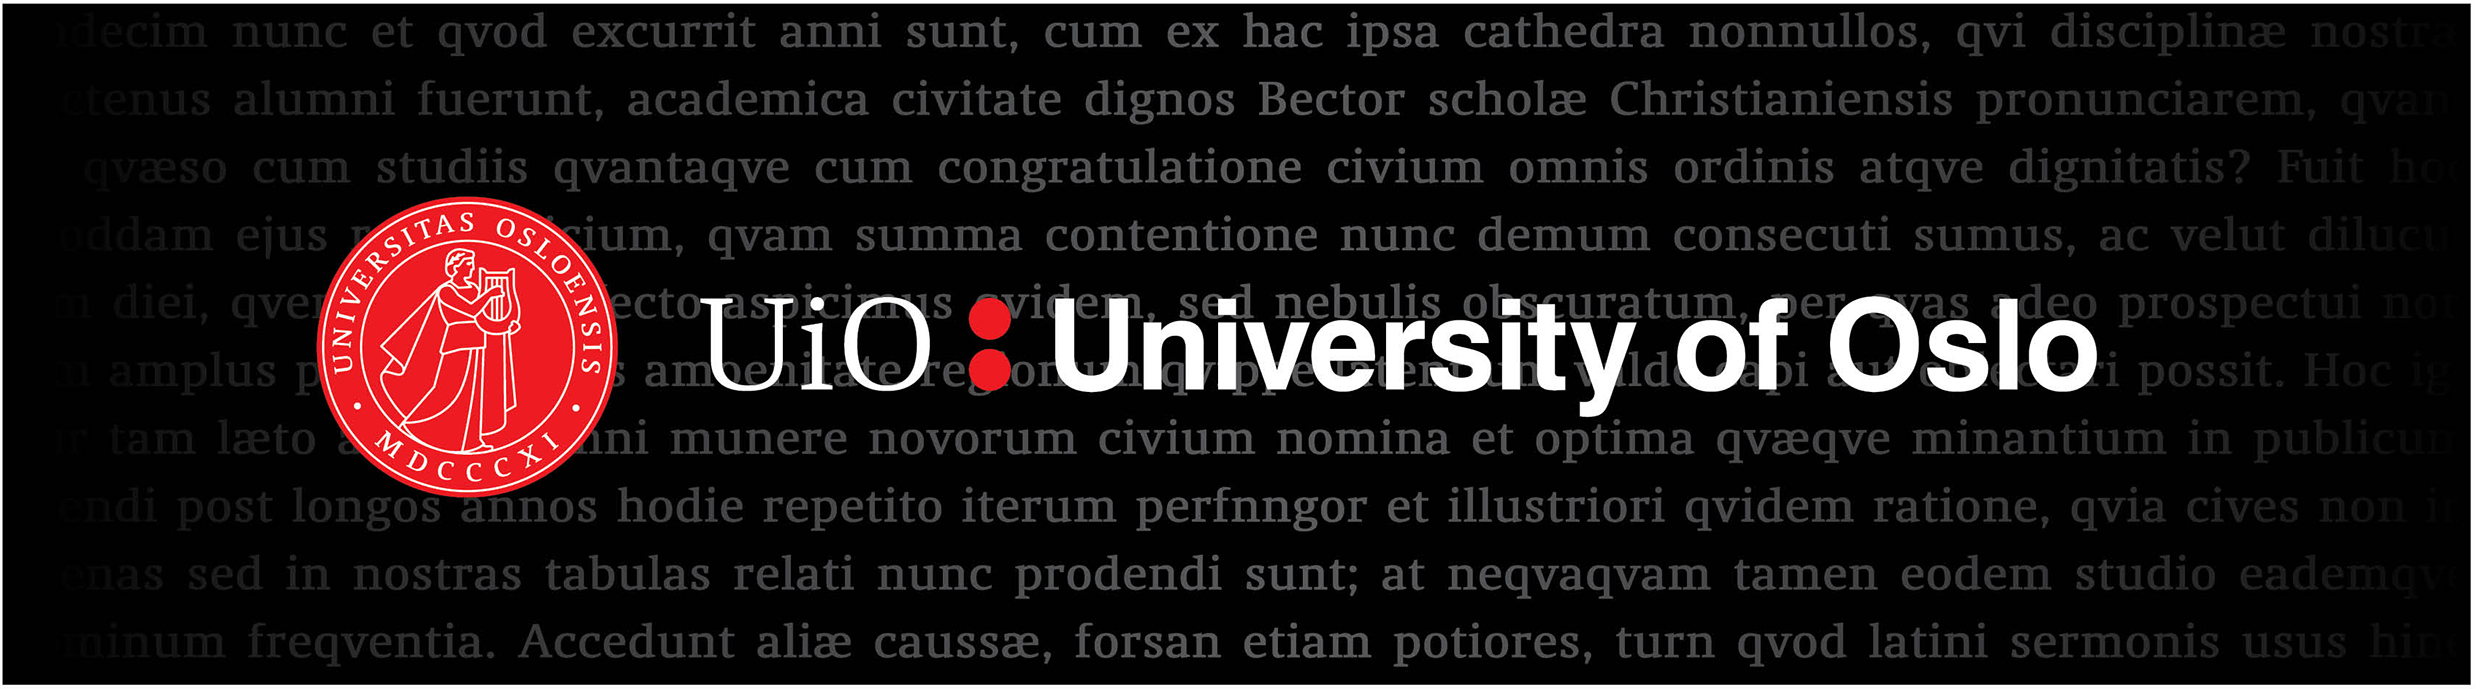
\includegraphics[scale=0.5]{toppfelt-english.jpg}\\\\
Using sensor networks and cloud technology to manage water usage in agriculture.
\\\\
\large A technology feasibility study}
\author{Erlend Westbye}


\frontmatter
\maketitle
Abstract
\\\\
This thesis describes building a small scale wireless sensor network implemented using commodity hardware and open source software. The sensors monitor soil moisture and temperature and distributes the data to an application programming interface running in a cloud environment. The goal of the implementation is to answer whether this system is a feasible way to monitor and reduce excess irrigation in agriculture. The system collects, stores and visualizes data and can support high throughput of data. The research describes both the system design and the implementation in detail. As well as describing how the modern information paradigm cloud-computing can aid in the development and deployment of the system described in this thesis. My evaluation describes how the implemented system is a feasible way to address excess irrigation, and describes why I think water management in agriculture is an information and management problem above all else. Through this thesis I have demonstrated how technology can be used as an integral part of monitoring and improving excess irrigation.

\begin{figure}[h]
\caption{Hjemly farm Osen, Hedmark}
\centering
\includegraphics[width=12cm]{DSC00258.JPG}
\end{figure}
\tableofcontents
\linespread{1.3}

\mainmatter


\chapter{Introduction}
Strukturen over må selvsagt tilpasses det aktuelle problem og type oppgave, for deg er vel erfaringsdelen viktig, men kan kanskje si det er en slags «evaluation»?
Det kan være ok å sammenligne erfaringene med hva slag forventninger/hypoteser man hadde i utgangspunktet.
Hva var ventet? Hva var overraskende? Noen råd du vil gi ?
\\\\
motivation for the work, description of the problem, 
goal of the thesis (should follow from the motivation), 
approach (how you approached the problem)
research method (optional)
summary of results/contributions
structure of the rest of the thesis (not included)

\section{Why is high water usage a problem}
Many are like me and turn on the shower without giving much thought to the amazing innovation that has gone in to getting the water running through the pipes in to my apartment. But i got to admit, I think less about the water it self. Especially in a country like Norway where water is abundant, and there is no significant visible cost attached to turning on the shower as both water and electricity is cheap here.
\\\\
Although we rarely think about it water is a finite resource. Non frozen Fresh water makes up 0.76 of the world's water supply.\parencite{WaterinCrisis} This number really sets the amount of available water in perspective. We will not be arguing whether the commodification of water is the worst thing that can happen to modern society, whether the free market knows what is right for the world, or how much of a toll agriculture is taking on the atmosphere of the earth. Instead I will be taking a long look in to the feasibility of using modern technology to reduce water usage in one of the most water intensive industries; Agriculture. \parencite{WorldBank}
\\\\
Water is high on the agenda. The United Nations has a list of sustainable development goals, where water is one of the items on the list. The OECD has also put forth water as one of the important things to put on the agenda. In a 2018 note they also mentioned the gathering of information as one of the important steps in improving the situation 
\\\\
"Improve information systems on surface and groundwater quality and flows, help to assess risks, and implement programs tailored to specific challenges."
\\\\
Norges Bank Investment Management (managers of statens pensjonsfond utland) has also made sustainable water management one of their goals for sustainable investing. 
\\\\
"Companies should recognise the business’
water impact, commit to sustainable water
management and, as relevant, have a clear
water management strategy." \parencite{latex2e}

\section{Water around the world}
 During the summer of 2018 Norway experienced severe drought. The lack of moisture in the soil resulted in severely degraded yield in livestock feeds grass and grain. This lead to severe financial losses for farmers in south and middle Norway. \parencite{nve} So even water rich Norway has seen that we are not immune to the changing climate and the effect that water shortages can have on our domestic supply of agricultural goods. 

\section{Questions to be answered by this thesis}

\subsection{Introduction }
The biggest cloud vendor AWS in the world was started in 2006. \parencite{Gartner} In the last 13 years the rate of innovation in this space has been staggering. This is something I have seen personally in the time where I researched and wrote this thesis. When it comes to streaming large amounts of data I know that there are many vendors that have achieved this and there are many services for gathering, processing and storing large data sets
\\\\
Examples of massive data stream systems are found as an example within the financial space. Where companies like OneTick can offer solutions that can stream and persist every single trade that takes place on an exchange. This gives a good idea of the big data capabilities that are implemented in cloud. \parencite{OneTick} Cloud vendors provide services like hosted data bases, data streaming platforms and data lakes. Developers are getting used to having immense computing capabilities at their finger tips, and data streaming is one of the things that could be implemented in cloud.  
\\\\
Humans where at one point hunter gatherers and as a part of our evolution as a society we learned to domesticate plants and animals. The farming tradition in Norway is rich, and driving through the Norwegian country side shows the large focus we have had on farming as a nation. Farming is an area that contains some incredible innovation on many scientific fronts, we have modified the genes of plants to make them more drought resistant and resistant to pesticides. I would therefore argue that agriculture is an industry where technological innovation is ingrained in the activities that farmers take on every day.
\\\\
Farming equipment is going smart, we have seen international media coverage on farmers going so far as hacking their farming equipment. I would therefore argue that agriculture is an industry that would be happy to adopt new technology as we have seen them do many times over.\parencite{motherboard}
\\\\
This is the central question of what I explored, and I started out with the standpoint that from a intuitive point this is the case. The research paper presented by Amy Lilienfeld and Mette Asmild gave us a clear overview that in broad strokes water consumption is more of a management problem than a mechanical problem. Some interesting findings of the paper that helped build up our theory is the fact that the age of the farmer had more to say for the water consumption of a farm than the irrigation system suggesting that through "smart" management and digitization of this industry can have an impact on this industry. Mismanagement of water can lead problems such as over pumping of aquifers \parencite{LILIENFELD200773}, and water management in agriculture is an area I truly believe that information technology can be used for good.

\subsection{Using sensor networks and cloud technology to manage water usage in agriculture.}
\begin{itemize}
  \item Is sensor technology a reasonable way to address excessive irrigation
  \item Can a system for monitoring water consumption be implemented with limited resource use
  \item Can such a system be implemented as a proof of concept
\end{itemize}
Keeping these three questions in mind I will address and answer all of these questions. From an intuitive standpoint one could think that the answer to all these questions are yes. However I will prove that these things are not just achievable from a theoretical point of view. But also something that can be implemented.

\subsection{Approach}
I chose an exploratory approach where I wanted to gain insight in to what factors i could monitor and how i could architect a system that could support farmers in making good water management decisions. We chose the primary strategy of building out a proof of concept ourselves as well as researching the topic through exploring previous work on the subject. We even went to meet with a farmer to talk about monitoring and what factors are of interest to them. As well as meeting with a leading Norwegian manufacturing automation firm to learn about their sensor offerings as well as how they develop their monitoring platform.
\\\\
With this mixed approach of learning by doing and reading about the subject at hand I have become well equipped to talk about the challenges and problems to be solved to improve water management in agriculture. And how IoT and cloud technologies can help in improving the water usage in this sector.

\section{Personal motivation}
Thinking back to the technology i had available 10 years ago I know from experience that the available technology and services has changed. And i am sure that there are a few revolutions within technology that has enabled this thesis. The first is the cost and prevalence of micro-controllers. A micro-controller is a small general purpose computer that typically consume little power and can easily used in an embedded context. The two major micro-controllers the Raspberry-PI and the arduino both ship with "general purpose input output pins" (gpio) meaning that these boards can both process data from the real world and the digital world provided that you feed it with data using sensors. This link between the real world and the digital world is something i find deeply facinating and it is what truly led me down the path of becomming passionate about programming. Another revolution has come in the availability of on demand computing resources through what has been dubbed "the cloud". When I started programming in 2013, cloud was already established as a good way of hosting applications, and is the deployment model i have used for most of my career. Cloud is a true enabler of proof of concept implementations as the upfront cost of implementing advanced system is reduced drastically as you would typically only pay for the resources you actually consume.
\\\\
This fascination with cloud and combining the real and the digital world is something that has given me a lot to think about in the last five years. And the reason why i wanted to build this system is to investigate how I can leverage technology to improve and help managing processes around irrigation in agriculture. I had long had an idea of starting a smart farm at some point, and i think that this backdrop has given me ideas for how to implement this on in a small scale outdoor operations at my farm in Hedmark where my wife and I will grow grass for cattle feed and Christmas trees in the future. Although i did not own this property at the beginning of this thesis it has given inspiration and motivation through 2019 and I will go in to detail on how i envision deploying this system there in the subsection marked "deployment conceptual"

\section{Quantifying the requirements of the system}

The requirements for this system to meet the purpose of the thesis, and being able to answer my central questions are based on the challenges described in "vanning og systemer" in addition to technical requirements that I came up with in the design and planning of this thesis. The fact that the text establishes a baseline by looking at the best actors and using them as a benchmark is a natural choice when the cost of gathering data is high. I will prove that the cost of gathering moisture and general plant related data has been reduced significantly and a deployment should be possible across a wide range of farms, regions and environment to establish a baseline to compare excess irrigation to. I researching this from a technological stand point, an I will prove that it is feasible to gather, store and visualize moisture data.
\\\\
The system will also need to handle concurrent requests from a wide range of sensors at the same time. This is important for a production context as I do not want the data gathering APIs to be a limiting factor in the system. To achieve this we need a system that can scale horizontally and is primed for being hosted in the cloud.
\\\\
Documenting a low cost, high throughput system is an integral part of answering whether this system can be incorporated in the irrigation process and help farmers make better choices for water usage. The system will need to visualize the data to a standard where it is intuitive for a farmer to see the water needs of a plant.
\\\\
To summarize the system will need to be able to gather data at a low cost, handle a high number of sensors at the same time and visualize the data in an efficient manner. If all these are achieved I envision that this system can be an integral part in the management of irrigation for any farmer that uses it and contribute to reducing water usage in agriculture.

\section{Research method}
 I will conduct a feasibility study considering the cost of a rudimentary set up set up in both cloud and on premise. I have built my own monitoring system with cheap and commonly available hardware. I have also written custom software to get a grip on the amount of data a system like this would produce on a larger scale. Taking in to consideration what data is relevant, and how to gather data from multiple sources. We will look at the cost and technology considerations of this system. Other important factors is the importance of data accuracy and data integrity. I implemented a large portion of the system that is discussed in this thesis to learn about the networking and hardware challenges that comes along with a distributed wireless sensor network. As a part of this I also tested different cloud platforms to provide insight in to the pricing and resource consumption in the cloud. 
\\\\
In the end I found limited value in the actual data I collected, but in so far as answering the question of whether or not this system is feasible it helped build our conclusion. The value came primarily from the visualization platform that was built as a part of the reference implementation of this system. This yielded a clear picture of the state of our monitored plants, and gave clear insight that could potentially help with watering in a large scale agricultural set up of a similar setup.
\\\\
Setting up the sensor networks is a challenging task as you are doing the work of a programmer and a product developer at the same time. What I want to prove is that it is feasible to build this type of system yourself and that there is room for an open source alternative to the commercial products that we will discuss in this thesis. We sought out to learn about our subject by actually building a function prototype. It is one thing to read about prior experiments, but a whole other to build it out yourself.
\\\\
I also read and gathered information about similar systems as well as spending time looking at the state of the art open source and commercial products in this space. It is also important to mention the cloud aspect of this proof of concept as it is one of the key cost drivers. I have explored the use of the vendors Microsoft, Amazon and digital ocean. As well as doing a theoretical comparison of the deployment of the system on physical hardware

\section{Central findings}
\subsection{Software}
Through this exercise in exploring the feasibility of a large scale agricultural sensor networks I have discovered that this type of software can be implemented by developers with modest professional experience using open source frameworks and public information. The implementation overhead can be kept low as the software I built is based on open source implementation of different systems. As we see often with a systems development, the code-foundation is out there in the public via open source, and it is possible to combine in to new products in a relatively short time frame. However it is important to note that implementing software is never trivial it is important to acknowledge the community resources and open source software that helps developers along the way. One central finding is that the willingness to share information and help other developers is a major part of why it is possible to implement this type of software.

\subsection{Hardware}
The price of the hardware was the biggest discovery I made on the in the hardware portion of this implementation. The ubiquity and availability of fit for purpose and general micro-controllers has been a huge help in the implementation of this proof of concept. I found usage of the raspberry pi and the NodeMCU micro-controllers especially useful as there are active communities for both. As an example I got electrical engineering help via the internet on a forum by posting a description of a problem i was facing. This example shows the power that one individual is given in the hardware space through online collaboration and open source platforms.  Another key finding is that the power constraints became a huge roadblock for a proper battery powered wireless sensor network, and that this would require further work and expertise to get to a production ready state. I also found that the system could be implemented using commodity hardware bought from cheap sources, and the availability and level of service offered by platforms such as Ebay and Alibaba are a huge enabler when doing prototyping development where physical hardware is required. But when it comes to managing battery power and implementing a system using stripped down versions of the esp8266\parencite{espressif} the challenges are no longer trivial to a developer with basic knowledge of electrical engineering and move over to physical hardware manufacturing.

\subsection{Cloud}
I tested three different cloud vendors and found them all to be more that adequate for our purposes. Our primary implementation used a common Linux distribution (Ubuntu), MongoDB installed on said server on the platform Digital ocean. In later times I have also explored hosted services like RDS from AWS and documentdb from Azure. We found that the hosted services from Microsoft and amazon had an impact on the cost of implementing this type of system.

\subsection{Cost}
We where able to run a basic implementation for a low cost, and have kept it running at approximately \$ 5 per month. The hardware is also relatively cheap depending on the type of sensor used. With the most basic sensor described in this thesis I was able to keep the cost to approximately \$ 10 per mote, and with the more advanced sensor described later I was able to do it at about \$ 25. Ordering bulk quantities of the same hardware would yield a substantially lower price.

\subsection{Feasibility}
I can state for certain that from a technology standpoint this type of system is very possible to build and can be implemented without excessive technical competence, and without high development and hardware costs. From a water use perspective the answer is more complicated but I can say that based on the theory that water usage is tightly coupled to management routines we can argue that this would be of great help to farmers that want to monitor and improve their water usage.


\chapter{Background}

Knowledge that is needed for the reader to understand the thesis describing relevant methods, tools, techniques that can not be assumed to be common knowledge
Description of (some) related work and its limitations w.rt to the goal of the thesis

\section{Water management in agriculture}
Humans have cultivated crops for a long time, and depending on where you read we see numbers going as far back as 20000 years (The Origin of Cultivation and Proto-Weeds, Long Before Neolithic Farming). 
\\\\
I have chosen to take the following approach when looking at excessive irrigation. And we follow the definition of (Estimation of excess water use in irrigated agriculture: A Data Envelopment Analysis approach) "The application of more water than a crop can use". Following is a definition of precision farming "Precision farming explains yield variability at the field level as a function of variability in inputs, including irrigation water."<- this is a note
\\\\

The application of more water than a crop can use, or over-watering, is usually the result of lack of knowledge about soil water content or crop water demand \parencite{LILIENFELD200773} highlights the fact that knowing the moisture content of the soil could be integral in reducing the over-irrigation of crops. Quantification of the extent of over-watering has been shown to be very valuable. (quote) Further supports the claim that quantifying the soil moisture content would be a valuable tool in reducing over-watering in agriculture.

\section{An Introduction to central themes of research}
The Future Internet is pushing the world towards a state of ubiquitous computing, connectivity and sensing. The concept of Internet of Things(IoT) plays a big part in this paradigm shift. IoT explains the shift in the hierarchy of the Internet where the number of "thing" entities outnumber the number of human entities and makes humans the minority of generators and receivers of traffic. IoT also calls for an increase in Machine to Machine(M2M) communication. One of the most important technologies of the IoT is Wireless Sensor Networks(WSN). A WSN is ''a network of battery-powered sensors interconnected through wireless medium and is typically deployed to serve a specific application purpose''\parencite{Ojha2015662}. To fully benefit from the ubiquitous connectivity of the IoT computation power, storage and networking infrastructure must enter the equation. Cloud Computing offers these capabilities and the utilization IoT in conjunction with Cloud Computing is the direction the Future Internet is pushing. This combination of technologies could be applied in a infinite number scenarios for better monitoring, data collection, analysis, forecasting and decision making. Developments in technology and in the prices of Cloud services means that these technologies are now available to almost any business that can make use of them. Agriculture is an area where the potential is tremendous for these technologies to work together, especially from an economic and environmental stand point. Agriculture is an area which highly relies on the climate in which it operates and must therefor adjust to the shifting nature of that climate. Knowledge of this shifting nature is key for successful agriculture. Environmental monitoring, data collection, analytic, forecasting, automated systems for irrigation or fertilization, plant health monitoring and frost detection are all scenarios that apply for both conventional and urban agriculture where these technologies can supply crucial information for important decision making. In this article I will explore the state of the art of these technologies and how they could be applied in different agricultural scenarios. We start by exploring concepts like Cloud Computing and IoT before move on to specific technologies like WSNs and application level protocols and conclude the thesis with examples of these technologies' applications in agriculture.

\section{Wireless sensor networks}
Wireless Sensor Networks(WSNs) are “a network of battery-powered sensors interconnected through wireless medium and are typically deployed to serve a specific application purpose”[1, p68]. This type of network are applied for a variety of different purposes, including environmental monitoring, machine monitoring, safety management, smart buildings, and for many other purposes. For any application this type of network would be comprised of a variety of sensors, such as temperature, humidity and volatile compound detection.[3] Technological advances have made small, low cost, low power and highly customizable devices commercially available and has improved the viability of large scale sensing networks with a large number of intelligent sensor nodes. A sensor node, nicknamed “mote”, in a WSN typically equipped with one or more sensors, a sensor interface, processing units, transceiver unit and power supply [2]. 
\\\\
For many years the trend in WSN topology has been a network comprised of several motes and one or several gateway nodes. In this type of network the motes communicate with each other and the gateway node using a radio frequency communication technology like Zigbee or Bluetooth. The gateway node can have several functions including computation and internet connectivity. The motes in this type of network can not communicate with the internet directly and relies on the gateway nodes for this making the network a closed or proprietary system with limited communication to the external world. Current trends are pushing WSN in the direction of the Internet of Things(IoT) using the Internet Protocol(IP) to connect every mote to the internet [4]. Connecting individual motes to the internet using  IEEE 802.11(WiFi) enables the utilization of IoT platforms and other resources in Cloud services. Applying a gateway based architecture to an IP-enabled, WiFi connected WSN is a natural choice if the gateway node(s) are able to perform challenging computing tasks. This architecture follows the concepts of Fog Computing(or Edge computing). In Fog Computing... If your system demands both low latency and computation on large amounts of aggregated data, a Fog architecture would be a natural choice. 
\\\\
Motes can be arranged in different ways. Motes can send traffic through a gateway or a sink node which forwards it to the internet, or if the motes are connected to wifi, they can send the information directly to the internet themselves. Your network topology will be decided by the the sensing situation. If the motes are deployed in a controlled environment with short distances e.g. inside a building, where a Wireless Local Area Network(WLAN) is possible the motes can be connected to the internet using WIFI. If the motes are covering too large of an area or for some reason its not viable to use a WLAN, the motes can be connected to an gateway node using radio communication like ZigBee. If the distances are too great one can do a distributed zigbee network or have nodes communicate using GPRS. As we will see in one of the refrence projects.
\\\\
WSNs could be seen as a part of the Internet of Things(IoT).
\\\\
The main difference between a WSN and a RFID system is that RFID devices have no cooperative capabilities, while WSN allow different network topologies and multihop communication.[3]


\section{Is over watering a management or a mechanical problem}

It is also relevant to provide some context on the common types of irrigation systems that are deployed. These will wary across geographical locations, but it is from a intuitive standpoint fair to assume that irrigation is being done in a similar fashion across the world. I have decided to include the systems discussed in the paper by \parencite{LILIENFELD200773} as well as describing some of the  other common irrigation methods that I find. The two main differences are: Using rainwater and actual irrigation. 
\\\\
Rainwater irrigation is an important part of farming and following the weather has a high importance in farming. As an example drought can decimate the yield of a crop. We saw this happen in 2018 with livestock feeds like grass here in Norway. In these situation water management becomes especially challenging as wells and other natural sources of water can get depleted. Rain-fed farming is the natural application of water to the soil through direct rainfall. Relying on rainfall is less likely to result in contamination of food products but is open to water shortages when rainfall is reduced. \parencite{cdc}
\\\\
Irrigation systems include but are not limited to surface irrigation, sprinklers, drip irrigation, center pivot irrigation. The main differences for the types of irrigation is the precision of the irrigation, the cost and the labour involved in doing the irrigation activities. Intuitively I thought that there is a high correlation between the type of irrigation used and the amounts of water used. As an example you could think that any irrigation that involves flooding would result in excessive irrigation. But as argued by (Estimation of excess water use in irrigated agriculture: Data Envelopment Analysis approach) A major finding of the study is that there is only a weak relationship between irrigation system type and the level of excess irrigation water used. In particular, flood irrigation \parencite{LILIENFELD200773}
\\\\
This is interesting to our research case as the implication would be that the resource intensive and costly exercise of changing or replacing the irrigation system used would not automatically result in a reduction in water usage. This in our mind highlights that gaining insight in the actual water amount requirements over time could be very valuable input to the management process of a farm. One of  the challenges highlighted by the paper [] is that the gathering of agricultural data is very costly and inaccessible to a large portion of farmers. Given that this paper is already 10 years old, I would argue that the implementation I have demonstrated as working has brought the price of gathering this data no longer has a high cost relative to the price of doing mechanical upgrades to an irrigation system. Systems are not clearly inefficient and management may play a significant role in the levels of water use efficiency that can be reached. \parencite{LILIENFELD200773}
\\\\
The conclusion that the management plays a significant role in excessive water usage is especially interesting given that the primary goal of this thesis is to conclude whether or not a system for collecting and visualising water consumption using WSN and cloud is feasible. This conclusion by [] is a big motivating factor and gives a good foundation to discuss the feasibility and value of a system like the one I will lay out in the implementation and design portion of this thesis.

\section{Cloud Computing}
''Cloud computing is a model for enabling ubiquitous, convenient, on-demand network access to a shared pool of configurable computing resources (e.g., networks, servers, storage, applications, and services) that can be rapidly provisioned and released with minimal management effort or service provider interaction.''\parencite{Mell:2011:SND:2206223} This is the National Institute of Standards and Technology's(NIST) definition of Cloud Computing. NIST further define the concept with five characteristics, three service models, and four deployment models \parencite{Mell:2011:SND:2206223}. The five characteristics are:
\begin{itemize}
\item \textbf{On-demand self-service} A customer can provision computing capabilities at any time without any human interaction with the vendor.
\item \textbf{Broad network access.} Resources should be available for access from a wide range of devices.
\item \textbf{Resource pooling} The vendors resources should be pooled and served to customers based on demand.
\item \textbf{Rapid elasticity} Computing capabilities should be elastically provisioned to provide rapid scaling 
\item \textbf{Measured service} Resource usage should be monitored, controlled and reported providing transparency for both the vendor and the customer.
\end{itemize}

There are a multitude of different service models, but some of the prominent ones are the once defined by NIST:
\begin{itemize}
\item \textbf{Infrastructure as a Service(IaaS)} ''Provision of processing, storage, networks, and other fundamental computing resources where the consumer is able to deploy and run arbitrary software, which can include operating systems and applications. The consumer does not manage or control the underlying cloud infrastructure but has control over operating systems, storage, and deployed applications.''\parencite{Mell:2011:SND:2206223}
\item \textbf{Platform as a Service(PaaS)} A platform for application deployment giving the user the ability to deploy applications created using programming languages, libraries, services, and tools supported by the provider.
\item \textbf{Software as a Service(SaaS)} A software provided to the customer running on the vendors infrastructure. The application should be available from various devices.
\end{itemize}

The 4 deployment models are:
\begin{itemize}
\item \textbf{Public} This is a cloud that is operated by a trusted third party that handles all of the infrastructure and networking for the user. This means that all of the hardware is managed by the trusted third party.
\item \textbf{Private} This is a cloud that is hosted on hardware owned by a company or individual. Here the user would have full control of the hardware. Cloud does not imply that the servers are hosted off site, but these type of clouds are typically hosted in private data centers.  
\item \textbf{Community} A Cloud exclusive for a specific community of consumers. This can be organizations with shared concerns. It can be hosted by any of the organizations or a third party. 
\item \textbf{Hybrid} Here a mix of private and public cloud is used. This is a very common approach as it offers great flexibility. And is widely used as companies still have a lot of capital invested in hardware.
\end{itemize}
 
One of the key technologies that has made the modern cloud possible is virtualization. Computer virtualization refers to to practice of running operating systems on virtual hardware. This is achieved by splitting the resources of physical hardware between different instances of operating systems. This is done by installing software known as a hypervisor on the hardware instead of an operating system like Linux on a computer. The hypervisor allows for operating systems to be installed on top of the hypervisor, so that one machine or pool of resources can run many operating systems at the same time.\parencite{1430631}


\section{Internet of Things}
IoT is the concept of connecting “things” to the Internet to gather data and perform actions. Examples of uses for IoT range from manufacturing to agriculture. And the concept is often looked at as a way to connect everything from fridges to juice presses to the Internet. The recent development that has made IoT more available is the low price and number of of WiFi, Bluetooth and radio enabled micro-controllers.  This means that any sensors with a compatible interface can be connected to the Internet at a very low cost.
\\\\
The high volume and low time to market of many IoT products has presented a range of challenges like privacy and network security. There has already been large scale issues with connected appliances. The hacking of the connected light bulb Phillips hue is explained in this article \parencite{6997469} Despite these concerns the number of IoT devices is rapidly increasing. And we are seeing wide spread adoption in both industrial and consumer scenarios. 

\section{Wireless Sensor Networks}
Wireless Sensor Networks(WSNs) are ''a network of battery-powered sensors interconnected through wireless medium and are typically deployed to serve a specific application purpose'' \parencite{Ojha2015662}. This type of network are applied for a variety of different purposes, including environmental monitoring, machine monitoring, safety management, smart buildings and many more. For any application this type of network would be comprised of a variety of sensors, such as temperature, humidity and volatile compound detection sensors \parencite{s90604728}. Technological advances have made small, low cost, low power and highly customizable devices commercially available and has improved the viability of large scale sensing networks with a large number of intelligent sensor nodes. A sensor node, nicknamed “mote”, in a WSN typically equipped with one or more sensors, a sensor interface, processing units, transceiver unit and power supply \parencite{Gubbi20131645}.
\\\\
For many years the trend in WSN topology has been a network comprised of several motes and one or several gateway nodes. In this type of network the motes communicate with each other and the gateway node using a radio frequency communication technology like ZigBee or Bluetooth. The gateway node can have several functions including computation and Internet connectivity. The motes in this type of network can not communicate with the Internet directly and relies on the gateway nodes for this, making the network a closed or proprietary system with limited communication to the external world. 
\\\\
Current trends are pushing WSNs in the direction of the Internet of Things(IoT) using the Internet Protocol(IP) to connect every mote to the Internet \parencite{6064380}. Connecting individual motes to the Internet using IEEE 802.11(WiFi) enables the utilization of IoT platforms and other resources in Cloud services. In some cases applying a gateway based architecture to a IP-enabled, WiFi interconnected WSN can be the natural choice, especially if the gateway node(s) are able to perform challenging computing tasks. This architecture applies the concepts of Fog Computing.
\\\\
Fog Computing brings the resources near the underlying network \parencite{6984239}. Compared to the Cloud paradigm's centralized computing, storage and networking resources Fog Computing pushes these resources closer to the edge of the network, closer to the user. For a system that demand both low latency and extensive computation, a Fog architecture would be a natural choice. In context of WSNs this means utilizing a Smart Gateway \parencite{6984239}. As explained in \parencite{69842392} a Smart Gateway should be ''collecting the data and performing pre-processing, filtering the data and reconstructing it into more useful form, uploading only necessary data to the cloud, keeping check on IoT objects and sensors’ activities, keeping check on energy consumption of power constrained nodes of IoTs, security and privacy of the data, and overall service monitoring and management''. 

\section{Integrating WSNs with Cloud services}
There are two main approaches to the integration of WSN data with a Cloud service. Which one suits your network depends on the architecture of your WSN.
\\\\
The cloud providers AWS and Microsoft offer an IoT platform. Amazon's "AWS IoT", Microsoft's "Azure IoT Suite"(and the list goes on) both offers connectivity for most devices, graphic remote resource monitoring, data storage and analysis, data stream analysis, security and application platforms. These platforms offers a broad array of elastic resources and can be customized to accommodate a WSN. There are also more specialized services such as Thingspeak, Xively, Carriots and Kaa aimed only at IoT and might not offer the same underlying infrastructure as the big Cloud vendors.
\\\\
It is also possible to create a more ad-hoc solution using the resources of the Cloud. Using IaaS services from a Cloud provider it is possible to create a service with the specific resources the network needs. K. Lee \textit{et al}. \parencite{5678063} explores a Cloud service for WSNs built on Amazon EC2 virtual machines. The article demonstrates ''how sensor networks can be combined with Cloud Computing to allow the offloading of resource-intensive tasks to the Cloud.''\parencite{56780637}.

\section{Application layer protocols}
One of the key issues in IoT and WSNs is power efficiency in devices, given that a large scale deployment would be severely compromised if the batteries of the nodes in the network had to be replaced often. Application layer protocols has an impact on power consumption as communication is the most power hungry task the devices perform. One must also keep in mind that packet loss can effect real time data analysis. These are issues to consider when deciding on a protocol. In this section I discuss the most common application layer protocols for IoT and WSNs.

\subsection{HTTP}
 
''The Hypertext Transfer Protocol (HTTP) is an application-level protocol for distributed, collaborative, hypermedia information systems''\parencite{HTTP1996}. HTTP is the dominating protocol for client-server application level communication in the Cloud context. However, HTTP has proven to be energy ineffective in constrained environments, in particular with the small frame sizes and the lossy links of low-power wireless communication that characterizes traffic from IoT devices and sensor nodes\parencite{karagiannis2015survey}\parencite{7030106}. Therefore, HTTP is seldom used in IoT and WSNs and the following protocols are preferable.

\subsection{CoAP}
The Constrained Application Protocol (CoAP) is ''a specialized web transfer protocol for use with constrained nodes and constrained (e.g., low-power, lossy) networks'' \parencite{rfc7252}. It was designed by the Internet Engineering Task Force (IETF) especially for devices with constrained resources. This makes CoAP a good option to use with IoT devices as they are usually resource-constrained. IETF state that ''The nodes often have 8-bit microcontrollers with small amounts of ROM and RAM, while constrained networks such as IPv6 over Low-Power Wireless Personal Area Networks (6LoWPANs) often have high packet error rates and a typical throughput of 10s of kbit/s.  The protocol is designed for machine-to-machine (M2M) applications such as smart energy and building automation.''\parencite{rfc7252}. CoAP runs over UDP in order to remove the TCP overhead and to reduce bandwidth requirements. The protocol enables RESTful communication in a client-server architecture with the well-known methods GET, PUT, POST and DELETE and can provide both synchronous and asynchronous responses creating painless interactions with HTTP in web applications.
\parencite{rfc7252}
\parencite{karagiannis2015survey}
\parencite{7030106}.

\subsection{MQTT}
Message Queue Telemetry Transport (MQTT) is a client server publish/subscribe protocol created by IBM with M2M communication in constrained environments in mind. It runs on TCP and is asynchronous. IoT devices are usually resource constrained, making MQTT a good option to use with IoT devices. The protocols publish/subscribe configuration demands less resources than request/response as clients do not have to request updates which decreases the network bandwidth and the need for computational resources. Comparing MQTT to CoAP we see that the UDP-based CoAP produces lower overhead than the MQTT which runs over TCP. However, because of the lack of TCPs retransmission mechanisms, packet loss is more likely using CoAP and with low packet loss MQTT can experience lower delays than CoAP\parencite{karagiannis2015survey}.

\subsection{AMQP}
The Advanced Message Queuing Protocol (AMQP) is ''an open standard for passing business messages between applications or organizations''\parencite{amqp}. AMQP originates from the financial industry has been reported to have an environment of 2000 user processing 300 million messages every day. AMQP supply asynchronous publish/subscribe communication and has a ''store-and-forward'' feature that makes it reliable even after network disruptions \parencite{karagiannis2015survey}. 
\\\\
IoT is still an emerging concept and therefore there are many standards trying to solve the same scenario. We see that cloud providers have support for a all of these standards in their IoT platforms.

\subsection{zigbee}
It is relevant to look at zigbee because it could have been a good choise for implementing a fog network where the sensor packages where radio based and where communicationg to the internet through an edge node in the network.

\chapter{Technology considerations}
I am partial to think that there is a “tech fix” to all of humanity's problems. And in this thesis I will argue that in the case of water usage, it is not just blind technology optimism. But a feasible way to help reduce water usage and alleviate some of the stress that is caused on our environment by agriculture. The main factors leading to this being more feasible now is the dropping price of computer processing in the cloud. Which enables us as computer programmers to churn through vast amounts of data and has enabled. And made machine learning much cheaper and more available to the masses. Another contributing factor is the dropping price of the type of hardware that is used in this proof of concept, as well as batteries which would help with making the motes wireless.
\\\\
Ultimately the goal of this system would be to identify a relationship between certain variables.  Given that the field of study we are in is not agriculture we will keep information on this subject limited, as I am focusing on moisture as the primary variable to measure. But one can definitely theorize that there is a multitude of variables you can look at. Some examples of values that can be read with sensors and cameras are ph-level of the soil, rate of photosynthesis, sunlight hours, temperature, moisture using fit for purpose sensors and ir-cameras for photosynthesis. If such a relationship between important agricultural variables could be established, you can use this type of monitoring system to aggregate trends on a farm, county or country level and say something about the optimal way of treating your plants within a region. We also theorized that over time as you identify the most important variables you could in principle start reducing the number of motes in the system and run predictive analysis on the data sets based on aggregate data for a region. One such factor could be weather forecast to analyse and predict the watering strategy that should be implemented for a farm, county or region. 


\section{Challenges related to throughput}

Any system that is processing large amounts of data will need to be able to process these data as they arrive. In our scenario we had five motes sending out data every 15-30 minutes. But we still spent time thinking about whether or not our approach is efficient at scale. We will talk about API scaling with different techniques as there are many ways to achieve good performance while still keeping in mind the cost of a system. As an example if we where to see that the API is not able to handle a high amount of concurrent requests we could deploy multiple copies of the API we developed behind some load balancing mechanism to achieve good horizontal scaling. Apart from this we also need to consider the following. How does our selected API middle ware deal with a high number of concurrent requests. How does our selected programming language deal with asynchronous requests.
\\\\
We also have major read write challenges transmitting our data. Do we want to transmit directly, or would it be more beneficial to group data in an edge node and transmit larger chunks of data. These are important things to consider as the ability to replay events and resiliency in the network is important to give a clear picture of the water usage in the monitored area. This will be covered more in the architecture and future work portions of the thesis.

\section{data stream management}
There are a number of things to consider when we look at the streaming system that is set up for this system. The main question one needs to answer when setting up a stream management system is whether or not you want to run queries on the live stream. In our case if we where to do a full implementation with analytics, notifications and real time visualization. One would need the ability to query the stream. One suggested approach is to use the offerings from the big cloud vendors. IoT gateway can feed data to a stream analysis service in azure and allows for real time querying of the data before it hits the database.
\\\\
I could have used a pub/sub pattern to subscribe to data arriving in the database. There are many frameworks which allows for notifying listeners when a new object arrives in the database. We experimented with facebooks graphQL specification implemented in node which allows for subscriptions to sockets that publish when new data arrives. This would not yield true real time analysis, however given the requirements described in the reference architecture one can imagine that true real time is not needed as the data we monitor does not have a tendency to change rapidly.

\section{Hosting}
The way to host is a major cost driver and to a large extent decides the feasibility for this type of set up in large parts of the world. And unfortunately we are seeing that the cloud capabilities in areas where water is the most scarce is not the best places to utilize cloud technologies. I have found that the system we built also could be hosted as an on premise application on a single network. In that case the cost of the system would be different, and could vary greatly in implementation cost based on the number of motes deployed.
\\\\
When considering a cloud deployment of this system the most important things to keep in mind is the network coverage. Which over most of Norway is good, this system could also be deployed using the 4g network as the data packet sizes are very limited. We can also cache the data from the motes on an edge node which can act as a gateway to the cloud, or in certain cases cache the data on the mote itself given that we use hardware with substantial amounts of ram and flash storage. For reference the esp8266 used for this proof of concept usually ships with 4MB of flash storage. \parencite{espressif}
\section{Power consumption}
We learned early on the the power consumption of the mote is hugely important and undoubtedly the biggest challenge while we where developing the motes used in this proof of concept. The longest life we where able to get using the "all in one" versions of the esp8266. But found that the unit is simply consuming to much power with its additional modules. We started to go down the path of trying to design our own low power implementation, but ultimately we decided that this was not the main focus of our efforts. However there are methods for reducing power consumption by keeping it in mind during development. And as you will be able to see in the attached code I have used  power saving functions that are built in to the "nodemcu" operating system that is loaded to the esp8266.
\section{Data integrity}
In my opinion the primary factor for data analysis is the overall integrity of the data-set, as this is what will be used for analysis of water consumption. That is why the main challenge for this system and the main consideration for our system is whether a cloud based database can support the integrity we will need to gain insight through using our data-set. 
\\\\
The secondary factor of data integrity relates to the connectivity of our sensors, and whether or not we are able to transmit precise and timely data for out monitored variables. In this case this has way more to do with the networking of our system and the way we program our motes. This will be covered in detail in the concrete implementation of this system.
\subsection{Eventual consistency}
The concept of eventual consistency would be followed for this type of system as you might end up with a data set distributed across multiple regions and a read and write specific database. Meaning that we would not necessarily need a always consistent model given that outliers would be weeded out if we normalize the data and that the event occurring between two data points would be from an intuitive standpoint trivial to approximate.
\section{scalability}
Any system gathering large amounts of data would need to be easily work at scale. There are a number of strategies that will be covered in the implementation notes, both for the concrete implementation and the reference architecture that we will present. One important concept is to keep state away from any interface that interacts with the database, and leverage the timestamps to do the heavy lifting of stitching the data back together. We will cover load balancing and stateless APIs in the section on how to achieve scale in a rest API.
\section{Data quality}
A key consideration is ensuring that the data is of high quality and that we can filter out the values that deviate too much. Over time the data sets will give an impression of normal values and through analysis it is safe to assume that I can filter out data that should not be a part of the displayed data. It is important to understand that it is easy for us to tell in a visualization when a data point is an unrealistic outlier, but it is better to have a version of the data set that does away with these data points entirely. One approach that could be considered is normalizing the data before the system sends it to the display component. Or implement a system that scans and cleans the data. In general I am more interested in keeping the data intact, as one could regenerate the same result again as long as the underlying data of the calculation is kept intact. This could allow for experimenting with different approaches for data quality assurance.
\section{asynchronous programming in web apis}

\chapter{State of the art and reference projects}

\section{Technology applications in agriculture}
TODO INTRO!!

\subsection{Automated Irrigation System}
J. Gutiérrez \textit{et al}. \parencite{6582678} has developed an automated irrigation system using a WSN comprised of soil-moisture and temperature sensors placed in the root zone of the plants. The systems consists of senor units, gateway nodes, the irrigation mechanisms and a web server hosting a web application. The sensor units communicated with the gateway nodes using ZigBee and the gateway nodes transmitted the data to the web server through a GPRS module via the public mobile network. The sensor units was powered by both battery power and solar power and contained the two sensors, a microcontroller unit and a ZigBee transmission unit. The gateway nodes contained a ZigBee module, a microcontroller and a GPRS module. The gateway nodes received, identified, recorded and analyzed the sensor data as well as controlling the pumps in the irrigation system.
\\\\
The motivation for the system was to optimize water use for agricultural crops in water scarce environments. During the 136 day test in a sage crop field the ??? showed ''water savings of up to 90\% compared with traditional irrigation practices of the agricultural zone''\parencite{6582678174}. J. Gutiérrez \textit{et al}. argues that ''the modular configuration of the automated irrigation system allows it to be scaled up for larger greenhouses or open fields''\parencite{6582678166} and that the system is ''feasible and cost effective for optimizing water resources for agricultural production.''\parencite{6582678174}. Figure \ref{AIS1} depicts the proposed architecture.

\subsection{Vineyards}
J. Burrell \textit{et al}.\parencite{1269130} focuses on how the agricultural workforce should play a role in the shaping of WSNs. The goal is to develop a WSN for use in a vineyard. The author has a human-centric research approach and use ''ethnographic methods including interviews, site tours, and observational work to broadly understand the work activities and priorities of the various roles working in a vineyard''\parencite{126913038}.

\subsection{On-farm frost monitoring}
F.J. Pierce \textit{et al}. \parencite{PIERCE200832} describe ''hardware and software components of technologies developed for regional and on-farm sensor networks and their implementation in two agricultural applications in Washington State, an agricultural weather network and an on-farm frost monitoring network''. The objective of the work was to use the technologies to improve ''important farming operations that add value through improved efficiency and efficacy of targeted management practices''\parencite{PIERCE200832}. For the on-farm frost monitoring network the authors implement a radio based star topology telemetry network and a ad-hoc software solution to collect, manage and display the data. The authors cooperate with the farmers to determine the requirements of the system. The system needs to ''report air temperature every minute to a computer operating anywhere on the farm''\parencite{PIERCE200832}, it was important that ''multiple workers involved in the frost protection event be able to view current and trend data for each monitoring station in real time''\parencite{PIERCE200832} and that ''The user needed to be able to set temperature thresholdsthat would trigger an alarm at their computer''\parencite{PIERCE200832}. Although meeting some problems with weather and the radio communications, the WSN helped the farmers make more informed decisions about what to do when the frost occurred. 

\subsection{Aquaponics}
P.C.P De Silva \textit{et al}. \parencite{7780266} has applied an IoT architecture to water quality control in an aquaponics system. Aquaponics is a soil less growing method in which fertelizer is created from within the system boundaries using fish waste. In this context the food production process is treated as ''a distributed industrial manufacturing process with strategic data acquisition, automated optimal control, and automated process control which is to be implemented in urban and rural areas.''\parencite{77802661}. The system is comprised sensor and controlling units denoted as endpoints, an an IoT cluster, a  streaming analytics server and an data analytics server. The system is intended to facilitate for urban agriculture and addresses food security issues for crops produced intensively in limited spaces.  


\section{Off the shelf hardware and software}
In the world of computer hardware and software we tend to see leapfrogging in technology which yields great results. One such revolution has happened within sensors and sensor networks, is the high availability of general purpose, small computers like the raspberry pi or the Arduino. As well as the falling price of fit to purpose sensors like the humidity sensors I have utilized in my proof of concept. This enables researchers and entrepreneurs to rapidly prototype and test hypothesis with hardware that used to cost hundreds of thousands for a fraction of the cost. This has fueled a plethora of easily configurable software and hardware. And spawned a sub culture of what we call precision farming enthusiasts online. 
\\\\
When it comes to the commercial side of this type of technology, this market seem to have gotten more mature recently. And there is a lot of content about this type of technology as well as commercial implementations of similar technology.
\\\\
There are examples of commercial operators in this space and in this section we will have a look at some of the operators in this space


\section{Off the shelf hardware}
There is not that many off the shelf hardware in so far as ready made packages that i have found during my research for this thesis. Most of the moisture sensors that are commercially available are manual read out sensors that tell you when to monitor. The same sensors that where used for this proof of concept is in my experience what comes up when searching for  of hardware. There are however different types of this sensor that have other capabilities than the ones used in the proof of concept. These are very generic, so I have not been able to find a spec sheet for the sensor. But it is hard to gain insight in to how they work compared to as an example the sensorion sht11 sensor\parencite{sensorion} where you can read the full spec of how the sensor works without being a customer of the company. In comparison we can refrence back to the sensor offerings from Bosch and Schneider where there is no concrete technical data easily available to the general public. I acknowledge that these companies produce hardware for a different customer segment. At the same time it makes it hard to do a objective comparison of the sensors mentioned in this thesis and the commercial offerings from these companies.

\subsection{Inmtn}
"Inmtn" is an industrial company focusing on among other things irrigation control. They have industrial scale solutions which is used for monitoring the factors that we where able to monitor in our proof of concept. This company utilizes a more generic type of control architecture called SCADA.  of architecture focuses on the entire production process instead of only the gathering of information like I have focused on in our proof of concept. [add source]

\subsection{Schneider}
Another more well known company that offers products and solutions similar to inmtn is Schneider electric. They have also built out a suit of tools for monitoring in agricultural applications. Schneider offers products that have taken the systems discussed in this thesis to a production level. As an example they offer hardware that integrates with existing controls for irrigation systems. They also offer systems for soil moisture monitoring that monitors some of the same variables discussed in this thesis. Interestingly they have opted for burying the sensors at multiple depths, and are also utilizing cloud services in the operation of their platform. Per November 2019 you can see a demo at https://scadafarm.azurewebsites.net/home . 

\subsection{Wildeye}
Wildeye is a company that seemingly focus on smaller operations as one of their key selling points is the price of their hardware and software. Their solution looks similar what I have outlined in my system implementation proposal. They have weather proof sensors which are wired to a central computer which distributes the information wordlessly. This differs from our proposal as you are not running a wireless sensors alone, but in tandem with other sensors. [add source]

\subsection{Bosch}
Bosch also features smart agriculture as a part of their website. It seems that this company is to a greater extent in proof of concept mode, given that they already create advanced tools it is safe to say that they will probably launch more tools in this space.


\section{off the shelf software}
The off the shelf softeare in this category can be split in to two specific product segments IoT platforms and dashboard products.

\subsection{tableu}
One example of a tool that allows you to view aggregate data and build dashboards is Tebleu. This software allows for connectivity to different data sources like csv, sql, ssas, odata and more. This is a very useful tool for generating views for data and is widely used within reporting in the financial sector. In our scenario one could imagine that a service that could be offered to farmers is creating dashboard views and reports using Tableu and I think  of software could accelerate the insight gained from the data I have gathered from the sensor network. One massive drawback to this product is that the licence is more that \$ 800 per year as it is heavily geared towards enterprise users.

\subsection{veracity}
Veracity is another example, but this is a platforms that crosses the gap of iot and dashboard and BI tool. This is a platform developed by Det norske veritas and is used for a range of industrial applications. Although agriculture is not one of the use cases mentioned on their website. I know from experience that sensor data is one of the strong points of this platform. This platform also has an active community that creates third party applications that can be leveraged to accelerate the insight and analysis process. 

\subsection{IoT hub}

\subsection{Powerbi}

\subsection{Konsberg}

\chapter{Cost constraints}

\section{Cost and context}
Without getting to philosophical we need to consider the simple question: What is expensive? This is important as it sets the context for the discussions that will follow in this chapter. We will be looking at costs in two different ways, what is the cost to society, and what is the cost measured in monetary value. Focusing mostly on the latter. 
\\\\
It is clear in my mind that excess water usage has negative externalities and costs to our society. Consider the  example of drought in Norway during the summer of 2018. Although edge cases to a certain extent now, we still need to consider the negative effects of excess water usage, this is mainly to understand why reducing water usage in agriculture is important. Depleting groundwater can also increase inequality as it can quickly turn in to an arms race where farmers drill deeper and deeper looking for water.
\section{Considering the world wide availability of the internet}
There is a discrepancy in the availability of internet connectivity in the developed and the developing world. And although this is improving over time with adoption of 4g/5g and investment in internet and communication infrastructure. This is a major hurdle that could face the implementation of a WSN system in certain regions of the world. And unfortunately the areas that are especially drought prone can also have other challenges on the infrastructure side. The solution I have presented assumes a certain level of development within telecommunications and internet infrastructure that is not available through the entire world.
\section{Cost of hardware}

Price examples from alibaba per nov 19

\begin{center}
 \begin{tabular}{||c | c||} 
 \hline
 Component & Price \\ [0.5ex] 
 \hline\hline
 NodeMCU & \$ 2.35 \\ 
 \hline
 Generic moisture sensor & \$ 0.50 \\
 \hline
 STH11 & \$ 12 \\
 \hline
 3v 1200 mah battery & \$ 3 \\
 \hline
 ESP8266 & - \\ [1ex] 
 \hline
\end{tabular}
\end{center}

Depending on the version of the sensor that is chosen one can see that the impact to the price of the sensor package greatly. I would argue that the information from the generic sensor that measures Resistance in the soul is interesting enough to warrant building a package containing just that sensor. My total cost where similar for a portion of the packages that where built later in the project as I ordered more of the components online. In the initial part of the project I purchased the components through a Norwegian retailer at approximately 3x the price. In the end i think that the listed prices based on the retailer Alibaba gives a more realistic picture of what the cost of implementing one sensor package would be. All in we built the deployed sensor package for 5.75 \$ with a battery and approximately 2.75 \$ without a battery. Which was incidental the configuration I ended up deploying. I have excluded the price of cables and power bricks as I had this equipment already, but the price of these components is assumed to be a low portion of the overall cost of the system.


\begin{figure}[h]
\caption{Nodemcu and Nodemcu schematic}%
\centering
    \subfloat[Nodemcu]{{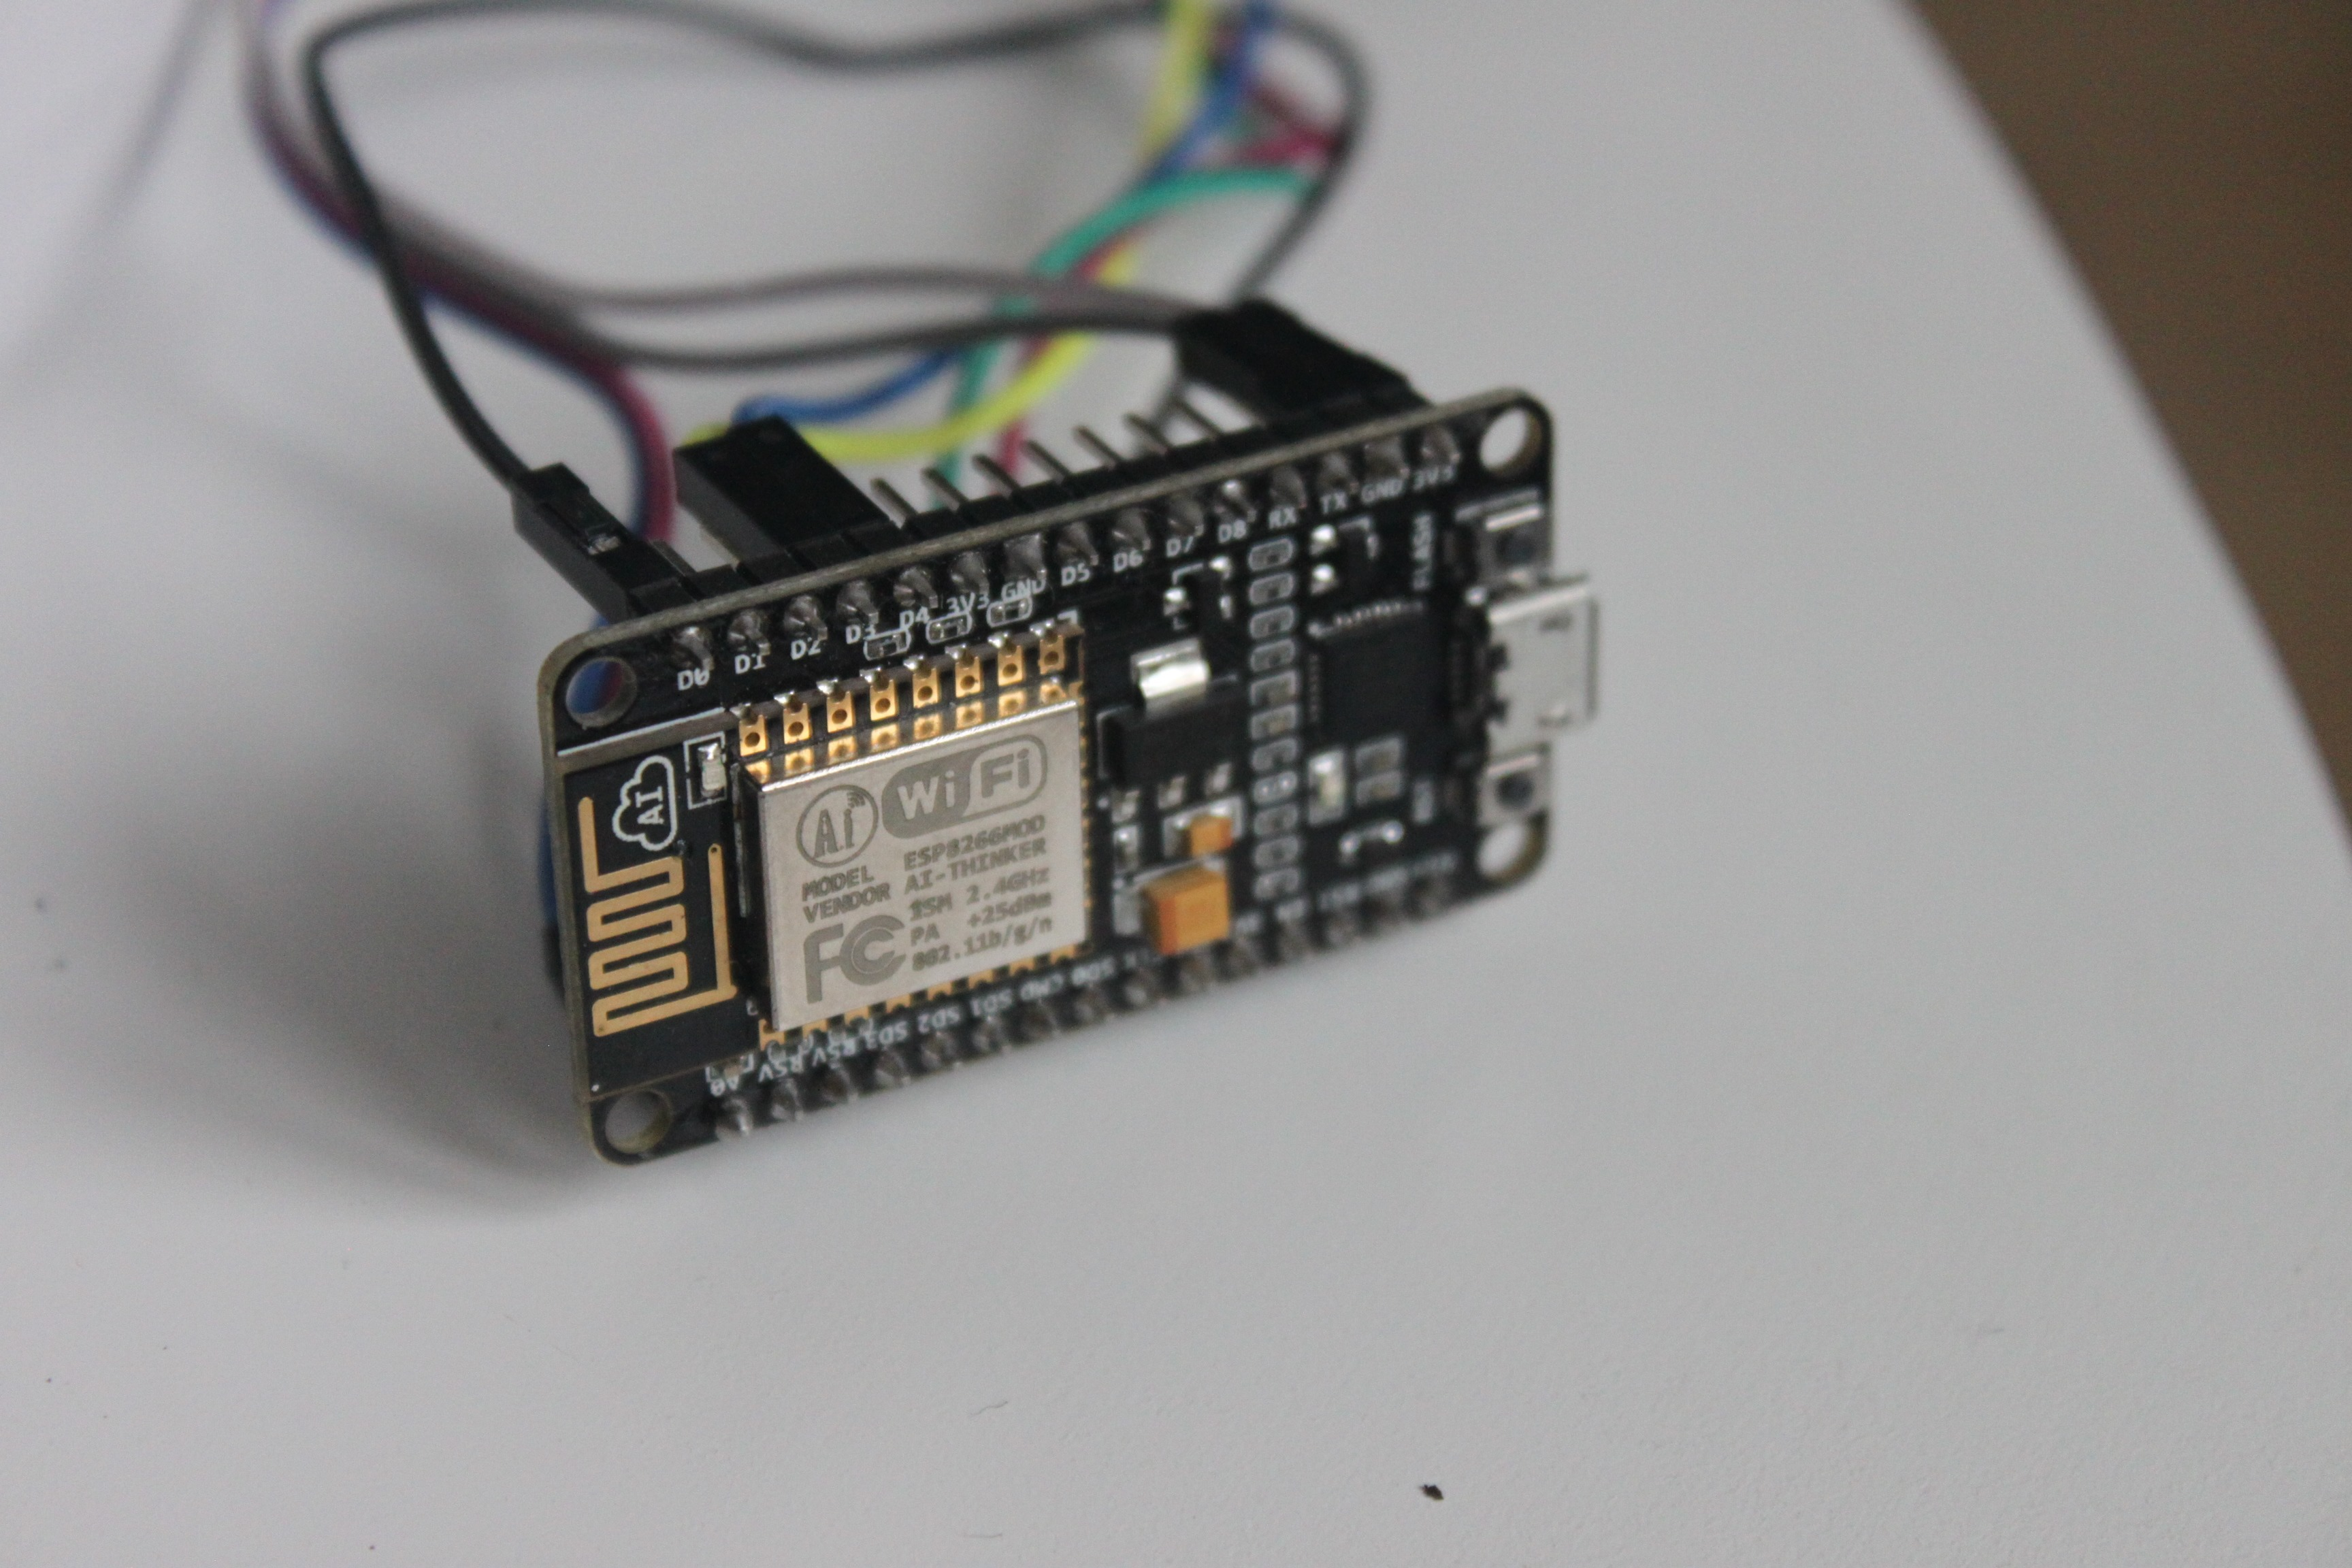
\includegraphics[width=6cm]{nodemcu.jpg} }}%
    \qquad
    \subfloat[Nodemcu schamatic]{{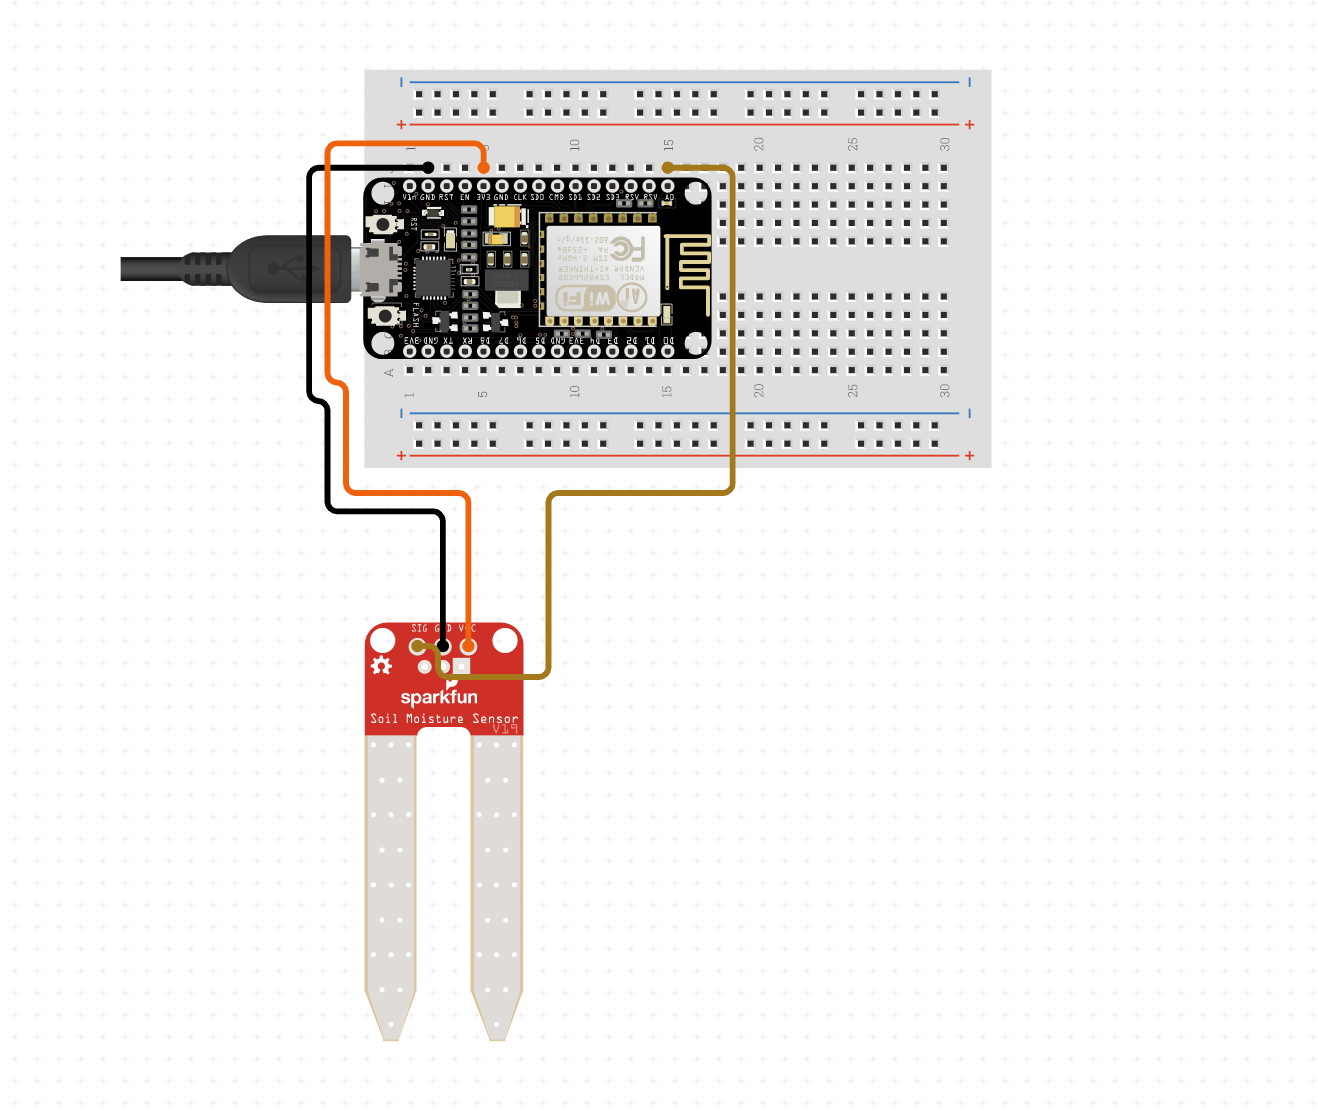
\includegraphics[width=6cm]{nodemcu_schematic.png} }}%
    
    \label{fig:example}%
\end{figure}

\section{Cost of hosting}
The cost of hosting is highly linked to the architecture that the application is designed around. Consider the following, redundancy, managed services, hardwere needs. All of these factors will play in to what the total cost of the system will be. To keep things simple and realistic for the purposes of evaluating realistic costs for the proof of concept system we will adhere to an three tiered architecture with the following components. Database, backend-API and front end view. I will review two different scenarios using IaaS and PaaS. For IaaS we will assume that one server is sufficient to host Database, backend and frontend. For PaaS we will assume that it is sufficiant to use one hosted web app container and one hosted document db solution. For the PaaS it is most applicable to review AWS and Azure as I dont have personal experience with the offerings for hosted services in digitalocean as they did not offer any that suited my needs at the beginning of this thesis.

\begin{center}
 \begin{tabular}{||c | c | c ||} 
 \hline
 Provider & VM INSTANCE & Price/month \\ [0.5ex] 
 \hline\hline
 DigitalOcean & small droplet & \$ 2.35 \\ 
 \hline
 Azure & linux vm &\$ 0.50 \\
 \hline
 AWS & ec2 t1.micro &\$ 12 \\
 \hline
\end{tabular}
\end{center}

Given the architecture that was implemented the cost breakdown would have been the following for the three hosting platforms that I investigated. One reflection is the fact that AWS and Azure offer more ancillary services and would probably have made future imporvements to the platform easier to implement. As an example there are excellent packages for application monitoring and usage statistics in both aws (cloudwatch) and azure (application insight) which are not present on digitalocean. So the total value of the Azure and AWS platforms are increased by the boundary resources that are offered by the platforms. In a production system the increased price of aws and azure could very well be worth it as the service ecosystem is more mature. 

Although the IaaS deployment model described above was what I ended up implementing. I still looked at service offerings from especially azure. In my opinion this is also a very valuable way of setting up the architecture of the application. One of the main benefits is the ease of deployments. This is again where the boundry resources of the platform giants are outshining IaaS provider digitalocean. As an example azure offers what at the time was called VSTS (visual studio team services) which allowed for very simple and straight forward ci/cd (continous integration/continious delivery) which is a fully automated way of deploying code to a production environment. This is another case of a platform having its perceived value increased by offering ancillary services to the end user of the platform. 
\\\\
The conclusion when comparing these platforms is that it is very hard to decide what to use based on price alone, like with any product, there is a whole host of things to consider. During the implementation of the project I found limited value in spending time investigating the minor pros and cons of each platfrom. An I am sure that they are all sufficient for the needs of the proof of concept I developed.

\section{Deployment context}
I have mentioned that there is a difference between a proof of concept project and a deployment context. What I mean by this is that the costs i can talk about are the once that I gained experience with during the implementation phase of this proof of concept. What we saw is that the cost of our system grew in a linear fashion for the motes. And in a tiered manner for the server costs, this is highly dependent on what cloud provider you choose but the following would be true for all of them. The important first step is to establish a baseline consumption of computing power. In the case of the proof of concept implementation, I chose the cheapest server available and that proved sufficient for the full implementation. Normally one would scale up by adding more machines to the pool of workers in the application. When you run on dedicated servers you would see that there is not a linear relationship between the amount of motes and the cost of hosting. Normally we would hit a threshold for capacity and then provision more hardware based on the increased need.
\\\\
If I had used a service from one of the major cloud providers for API management and databases the cost picture would have behaved completely differently as there is a high chance that the number of requests and amount of data stored would have more to say for the cost of operations of the system.
\\\\
If we where to deploy this in a production setting you would be looking at a set of other cost drivers which are not accounted for in this proof of concept. But from a host perspective it would probably look mostly the same. I envision that it would be benefitial to leverage more hosted services as ususally the bigger cost driver would be paying the engineers that are creating the application, which was not a factor in my implementation. At that point it would make sense to take a serious look at the differnt hosting models for cloud.
\\\\

\section{Summary}
As we have seen it is important to scope and explain what expensive is based on the deployment context. Given that I have researched this in a Norwegian contex, I would say that the cost critaria of the proof of concept has been interesting to look at. The hardware cost is experiencing good synergies from open sourcing and cheap shipping from china. The hosting cost are being pushed down by a highly competetive marketplace where providors offer good rates for computing power. The software packages that was used in this proof of concept where open source and contributed greatly in accelerating the implementation of the proof of concept. As far as achieving the requirement of gathering and storing the data in an inexpensive way I would argue that the cost break down shows that it is possible to argue that this the system outlined in the proof of concept could be implemented at a low monthly rate.


\chapter{Implementation and evaluation, An overview of a proposed implementation}

Sometimes split into two chapters depending on complexity etc.
(Discussion and) Description of implementation choices made 
Evaluaation: description of the experiemnts taiming to show the properties 
and performace of what you implemented in relation to the goals (how do you show that you have reached the golas of the thesis)


\section{Design}

Goal of the design
Discussion of design choices
Design details

\section{Describing an ideal system design}
\begin{figure}[h]
\caption{Reference system design}
\centering
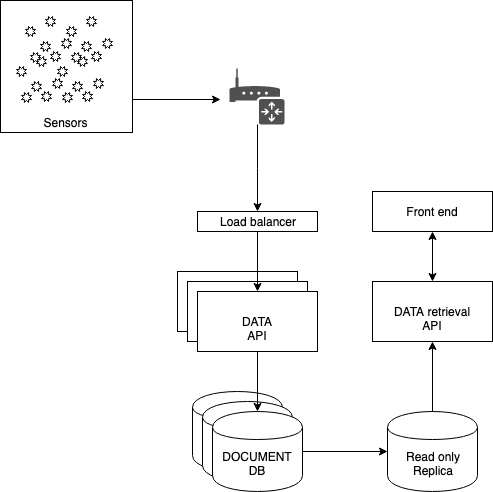
\includegraphics[width=8cm]{ideal_system_design.png}

\end{figure}
Early on I had a clear vision on how to build a system that scales well when the amount of traffic. That can handle multiple user sessions without impacting the performance of the data gathering APIs. Figure 3.1 is an illustration of the reference design that I started building our application based on. This diagram omits any gateway or edge node in favour of a system where I assume that we have good networking coverage.
\\\\
The data collected was initially limited to only moisture, this was interesting as I could see the plants consumption over time. A challanging part of the beginning of the proof of concept was figuring out what thresholds should be set for watering. I quickly realized that the system I had envisioned was ignoring factors like evaporation and we explored the possibility of also monitoring the temperature of the soil in addition to the moisture level. This data proved very interesting as we could see a clear correlation between temperature and the rate of evaporation of water from the soil that was monitored.
\\\\
Ultimately I realized that I had taken an oversimplified view of what is important to look at when you try to understand the complex picture of plant health. But I also realize that water is the primary factor that we would like to monitor, and I saw that the data I was able to capture gave a good picture of the water consumption and I do theorize that this data can do a lot to cut down on water usage in agriculture.

\subsection{Load balancer design}
A load-balancer would be responsible for unifying all of the stateless apis and exposing them as a single DNS address. As an example we could have a website like example.com point to a single machine/ip. Or we could have the same address point to a load balancing server/service that divides the load between a number of the stateless API. A load balancer typically works on a algorithm to assign requests to any of the APIs in the system. A common example of this type of algorithm is round robin. This would be a good strategy for handling load increases as more and more instances of the stateless APIs can be added to the load balancers list of available workers.

\subsection{API design}
We assumed an API first approach where we need to think about the resources that we will need in the API. As an example we approach the API design by breaking down the model of the objects that would need to be contained within our system as this quickly can give a good impression of the resources that we will need to create, read, update and delete. Generally web-API design has a clear segregation between resources by implementing controllers that have very specific jobs. This is a design pattern that lends it self to document based storage solutions as the objects and resources that are accessible through the API, are typically very similar to the schema of the database. A good api design will lay  the foundation for meeting the reqirement of the system being able to handle a large amount of data from a sensor network. Web APIs are built to handle a large number of concurrent requests at random intervals, such as retrieving data for displaying products or news to users. This is valuable as the requirement for the system is to handle a large amount of concurrent requests. To ensure that any request can be processed regardless of data arrival order we ensure that the design of the API stateless. A general observation is that this is easy to achieve when the API is responsible for creating entries and these entries are timestamped. This allows me to offload the ordering of the data to the client, and ensures that each request will be self contained.

\subsection{Database design}
The database design is often based around how I choose to structure the data. And in our case I have a clear definition of what data points we want to gather and what the model for said objects would be. One thing to note is that through this proof of concept I always thought of my model as one that is a natural candidate for nested objects instead of a relational database. Working with document databases has a range of advantages that we knew about during our design phase. The implementation idea was to have a high performance implementation of MongoDB, and if we needed to we could add long term storage, and high performance caching to the read API. Another important concept of the design is the read only replica of the database to be used for the view portion of our application.
\section{Model design}
\begin{figure}[h]
\caption{Model design}
\centering
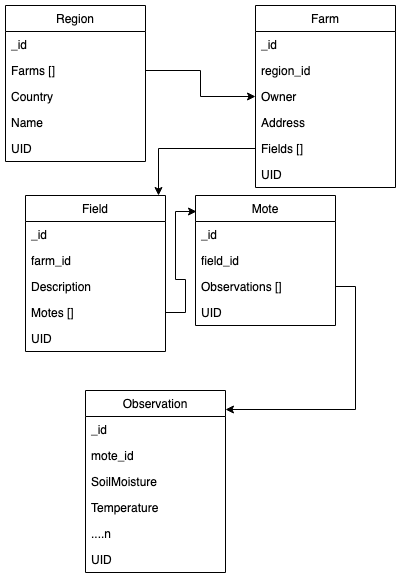
\includegraphics[width=8cm]{model_golden.png}
\end{figure}

The model design says something about the relationship between the different objects in our system and how they relate to each other. Here we focus on taking in a view of the whole system, and keep in mind that we would like to build a system that can scale beyond one single location. The design also takes in to account how the user can drill down from a farm level, or if the route is chosen, how interested parties can drill down in to the data from a region level. We envision that the proposed model design can ease the analysis of aggregate data, and at the same time provide the foundation for a fast and reliable way to update the database.
\\\\
While document databases are a good way to nest data in a manner that is logical given their relation. It is still important to keep in  mind what parts of the model could potentially slow down an insert if it needs to go through a lot of steps to reach its destination. As an example farm.mote.observation is a good way of finding data when you are in the context of a view. But when we consider the insert, it will be more beneficial to log an observation on the mote level, instead of considering what farm or area the observation belongs to first. This design challenge in the model could be solved by saving references to the different relevant IDs instead of embedding documents. In the API layer there has emerged technologies that abstracts away the embedding and allows the user to select whether they want to see the nested version of an object. GraphQL allows users to submit a schema that they are interested in, and as long as the API has definitions for where to look for the referenced objects it can pass back the full embedded document/nested object to the user. This achieves the same positive effects as the embedding, without the drawbacks of intermingling the objects.


\section{Implementation conceptual}
Cloud technology has enabled us to set up large scale systems at a much lower upfront cost, this is very advantageous in monitoring and ingesting large amounts of data. I would like to propose an architecture that I have found efficient and is a good fit for our application. 
\\\\
There are three main components that need to be considered and the first and most important is how we link our motes to the cloud. There are a multitude of concerns that need to be addressed like potential bottlenecks, security, and choosing the correct gateway for our motes.
\\\\
I have chosen to go with an architecture that allows the motes in the system to be highly autonomous/ low coupling and no dependency to each other. This is an choice that requires a bit more bandwidth usage, and is most advantageous when there are no caps, and the internet connection is not mobile..
\\\\
The point is to have every mote operating individually and having an isolated connection to our ingestion (platform/engine). This means that the motes have their own connection to a router and is free to communicate with the internet. This raises some challenges regarding security as a larger part of our sensor network is internet facing. This is something that would have to be treated carefully and given more thought in a production environment. This layer of the architecture also describes the network (layout/topology) and the structure that we propose for a multi site setup for precision farming as well as the network structure for our (demo/trial) environment.
\\\\
Each mote is connected to the internet via a normal wifi router. Every mote has an ip address, but you are not able to give our test kit remote instructions. Changes have to be made by flashing new software to the chip. Our motes acts just like any client on the internet and is able to send post/get requests just like a normal computer. This means that it is very easy to program the motes for any developer with basic web programming knowledge. The computing power requirements for the motes are very low as the system I have designed is intended to read data at a low requency. (test data collected at 30m intervals).
\\\\
The mote network fits the description of a star network where the common connection point is the router that gives access to the internet. There are multiple configurations that are relevant in an iot network, and star is one of the more rudimentary topologies. But in our case this is what makes the trial environment easy to set up.
\\\\
Ingestion is a very important component given that it would need to scale when more monitoring sites are introduced to the system. I have designed a simple ingestion engine to compare with cloud offerings from multiple providers. The ingestion is a one to many relationship and the data has a single point of entry. This is the same in both azure and our custom ingestion engine. There are many things to consider when creating the infrastructure to handle vast amounts of data, and the entire stack of the technology needs to be optimized in some way. A lot of the work in assessing the feasibility of iot in agriculture is selecting the right transfer protocols for optimal power consumption.
\\\\
 When the data has traveled from the “ground” to the cloud we are dependent on reliable and cost effective storage of the data. Given that many iot devices uses json to communicate with a server a natural choice for storing data is a json based document database like mongodb. This type of database is capable of many of read and writes per second. Due to the nature of our application write performance is the most important. One big advantage of cloud based data base systems is that they often do automatic replication over multiple locations something witch is great for data redundancy.
 
 \section{Site deployment conceptual}
 \begin{figure}[h]
\caption{Site deployment}
\centering
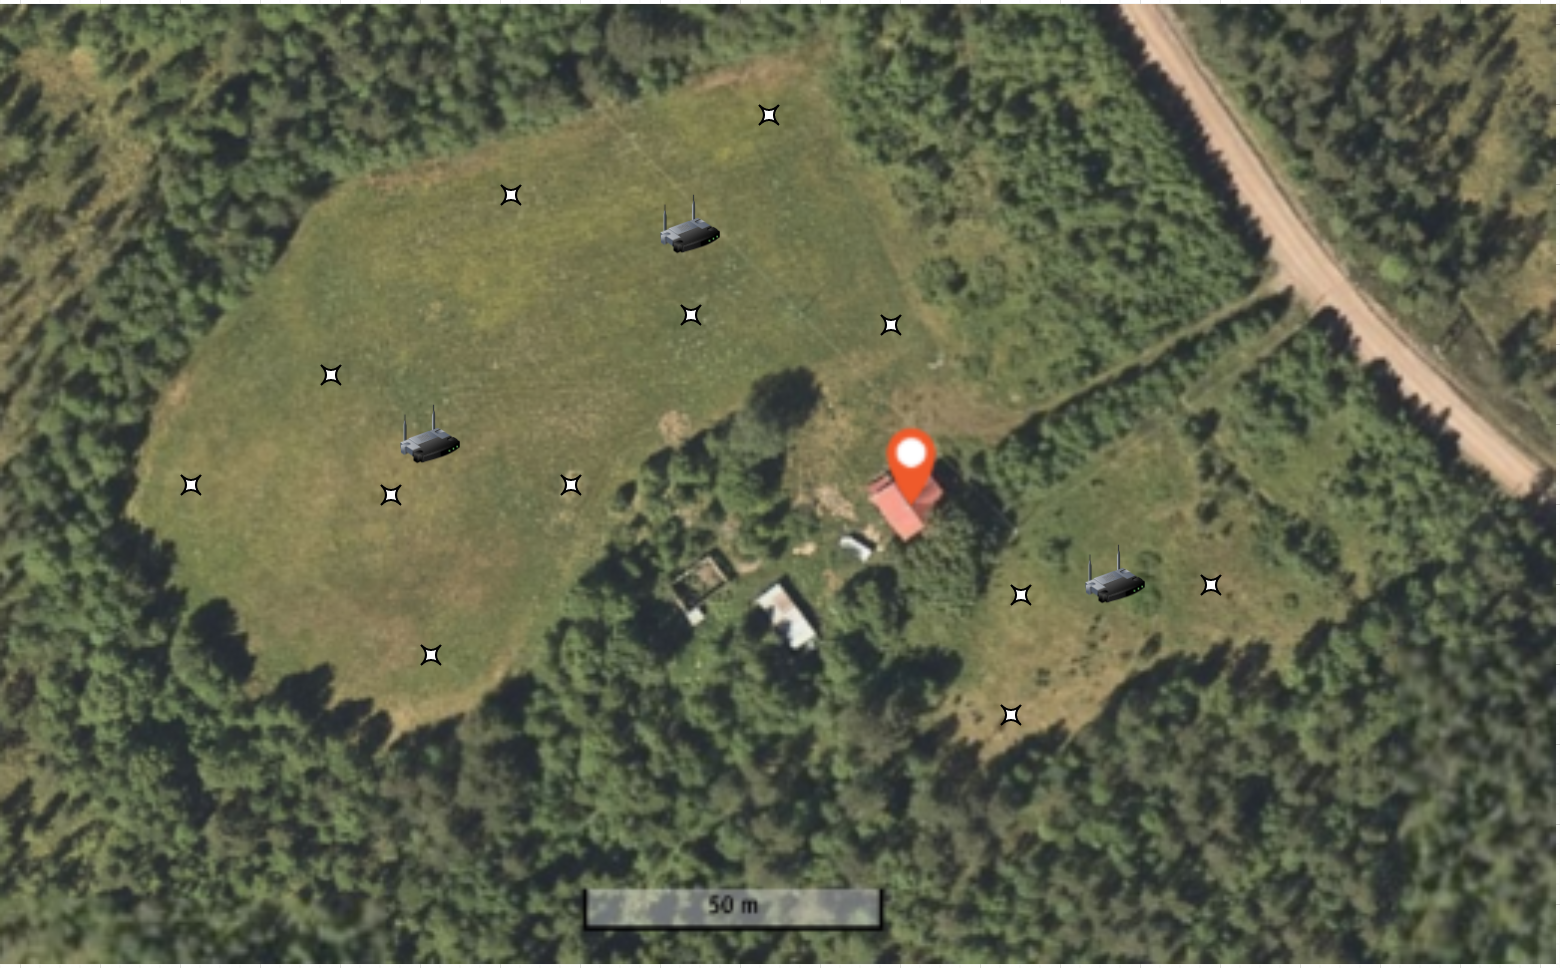
\includegraphics[width=10cm]{hjemly.png}
\end{figure}

 Following is a conceptual site deployment for monitoring a grass field of approximately 11ha, which incidentally happens to be the grass field of my farm in Hedmark. The idea is to think of this farm as having to "fields" and both fields being of interest. Why do we want to split these fields? We have observed that the yield is significantly different as one of these fields get a lot more sunlight than the other. It will also be interesting to describe how we theorize the networks requirements over such a spread out area.
 \\\\
 Field A is approximately 8ha while field B is approximately 1.5ha. To cover this entire area with wireless signal you will need to set up a network that can hand over connectivity in a seamless manner. We could go many different routes for the configuration. But we theorize that the easiest way to set it up is using repeaters for the signals. We would probably need to run power to some strategic locations in the field. Assuming a modest range of 150m we could in theory cover the field by using two WIFI access points, and with amplification we could cover both fields. Just from this exercise we see that networking could be a hurdle, but we are certain that this would not be a show stopper for gathering data as there are alternate ways of communicating via radio signal that I have not explored.
 \\\\
 When looking at the placement of the sensors we would consider the elevation, and the sun conditions in the patch we are deploying the sensors as seeing how much the reading vary would be hugely beneficial as it could tell us a lot about the amount of sensors we would need to deploy to get satisfactory readings. As well as some of the different areas of the field being more prone to retaining water and having different soil qualities. 
 
\section{Proposed solution}
Our proposed solution consists of a simulated Wireless Sensor Network(WSN), a real life small scale WSN and a cloud hosted web application. The simulated WSN is a representation of a general network of sensor nodes measuring soil data in an urban agricultural setting. The simulated WSN is based on data from a real life small scale WSN we implemented. This real life WSN consisted of nodes based on the NodeMcu development board which collected soil data our houseplants. The data was stored on a web server and later used to create datasets for the simulation. The WSN was active and collected data for several months. 
\\\\
The goal of the simulation is to test what kind of hosting service is nessecary.
\\\\
The solution is a testament to how minimalistic the application and interface part of systems with similar characteristics could be done. We host our application on a very affordable cloud service to insignificant cost and show that this kind of system can easily handle the kind of traffic a WSN produces. Based on datasets we produced in 2017 we can scale the WSN to stress test the web application. We will now talk about the data collection phase and explain our solution in greater detail.

\subsubsection{NodeMcu}
The sensor nodes are based around the NodeMcu development board. The NodeMcu board is again build around the ESP8366 WIFI chip. To develop an application for a NodeMcu board, you must first create the firmware for the ESP8366 chip. The chip comes with standard firmware, but for software development you need more libraries than the standard firmware. The firmware is modular and you can put together your own custom firmware using an online firmware build service called nodemcu-build.com. When you have flashed the firmware, you can write Lua scripts which you again flash to the chip. For our application, only very simple scripts are needed. For the nodes I have scripts which each 30 minutes reads sensor data from the analog and digital input pins on the board, creates a data-point and a HTTP request and sends the data to the server. When the request is sent, the device is set to sleep mode to save battery/power. The boards needs 3v power to run and can use both batteries and normal power.
\\\\
It is hard to run this type of board off of battery as there are quite many of the components that consume a lot of power. The esp8266 controller has a built in low power sleep mode which can be utilized for ultra low power operation. The problem for our poc is that the board that the esp8266 controller has many additional components like the USB (universal serial bus) controller mentioned above. This halted our progress for creating long running nodes in our system. But I managed to have it running for up to five days off of battery power with the nodemcu board. Proving that creating a completely wireless system is possible. We purchased the esp8266 board without the additional components of the nodemcu board, but completing the electrical component work proved to be more challenging than I first thought. And I decided on leaving that part of the project behind to focus more on the software and proposed architecture of this type of system.

\subsubsection{Sensors}
The nodes record data from a digital temperature sensor and an analog soil moisture sensor. The sensors are read by accessing the digital and analog input pins on the NodeMcu board to which the different sensors are connected. The soil moisture sensor measures the soil resistivity. The soil resistivity is the measurement of how much resistivity an electrical signal experiences travelling through the earth. The less resistance, the more moisture there is in the soil. The temperature is measured with a Sensorion SHT11, an integrated circuit which contains a silicon band-gap sensor. \parencite{sensorion}

\subsubsection{Creating data-sets}
Data visualization is an important step in showing the power of the data that I have gathered in the proof of concept I did. It illustrates that we are able to gather data the gives a good representation of the current state of a plant/patch of land. As you can see from the illustration underneath this type of data is very intuitive as evaporation is something that we are familiar with
\\\\
For our proof of concept I used two different soil moisture sensors. One is a very rudimentary sensor that measures the resistance in the soil between two metal rods. This gives a good indication of moisture level. Water is a good conductor of electricity which means that a reduction in resistance means that there is more water present in the soil
\\\\
The second sensor that I implemented is a humidity sensor paired with a special housing that allows for air to pass through, but not water. This means that as the soil moisture increases the moisture of the air that passes through the sensor. This type of sensor also contains a temperature sensor, which gives us valuable information of the current state of the soil that we are monitoring.
\\\\
We did not measure the sensitivity of our sensors, but to get a usable humidity readout I created a span between the readout from 100 percent humidity (sensor submerged in water) and as close to completely dry soil. For the humidity style sensor I got our baseline verification by checking that the sensor was within a few percentage points of the humidity reported by "metrologisk institutt" outdoor in the area that we where in.
\\\\
The resistance based sensor is analogue, and it is easy to read the information from the sensor. As it is connected to a pin on the board that is able to read resistance. The humidity sensor is digital and required that a library for communicating with the sensor was loaded on to the micro-controller. This type of open source software is often easy to find online for most types of micro-controllers. This also held true for the micro-controller that I was using (NodeMCU). As I found a Lua implementation that gave a good read out to establish a baseline for temperature and humidity

\section{Web Application}
The web application is a simple application built on the MEAN-Stack. The application receives and stores the data points from the WSN motes while providing a web interface. The web interface shows one graph for each area in the WSN. The graphs show the average temperature and soil moisture in that area for the last 24 hours. Each point on the graph is an calculation of the average temperature or soil moisture from all the motes. The interface is chosen not for actual use but as a proof that the web application can handle a certain traffic and functionality. 

\subsubsection{MEAN-stack}
The MEAN-stack is a combination of technologies that allows developers to create lightweight web application written in all Javascript. It consists of the four elements MongoDB, Express.js, AngularJS and Node.js. MongoDB is a noSQL database, Express.js is a server side javascript framework, AngularJS is a frontend javascript framework and Node.js is a server side Javascript runtime environment. 

\subsubsection{Database}
For our proof of concept I decided to go with a noSQL system. This is different from a regular relational database as the stored files are can handle nested object, instead of using a key relation as in a relational database. This type of system lends itself well to nested objects, as there is a clear relationship and tree like structure to the layout of the data model. Our data model was only concerned with storing the moisture data, and not the kind of administrative data that you might need for this type of system in the real world
\\\\
All calculations and data aggregation are done in the browser. We do this to offload the server, as I want the server to only handle the HTTP requests. The performance of the browser side application is decent, however the Javascript library used to generate the graphs have a lot of functionality, like animation that are not really necessary for this purpose, which gives a sub optimal rendering time. For this situation, a simpler library would be better, however the point of the web application is not to prove response time of Javascript libraries, the purpose is to prove the responsiveness of the server. We also want to point out that using AngularJS as the main front end framework is not the best fit for this application. For rendering of this kind of front end components(graphs) React in combination with other libraries would be a better choice. 

\subsubsection{Hosting}
For this proof of concept I have looked at the following vendors: Aws, azure and Digitalocean. The two former are the hosting giants Amazon and Microsofts offerings and is what is currently commercially viable for larger companies. And Digitalocean is a IaaS offering that is geared more towards the customers who are fine doing their own patching and upgrading. The three platforms also differ a lot in that AWS and azure offers a large range of software as a service, and Digitalocean only offers infrastructure as a service. We will also compare what offerings the vendors have for API gateways, storage {add more}
\\\\
We are hosting our application on a Digital Ocean Droplet. Digital Ocean is a cloud infrastructure company that offers affordable cloud services. A Droplet is a virtual machine instance with varying degrees of computing power, storage and networking functionality. We are hosting our application on the cheapest possible option. We use one Droplet with 1GB memory and 25GB storage. This is costing us 5 dollars per month, which is an insignificant expense. 
\\\\
Often there is no need for more than a simple server to run this type of application. But I also made an effort to explore alternatives when it comes to cloud hosting. We came at this proof of concept with cost as one of the key constraints that I have kept in mind. As this type of system would need to run at a as low as possible cost so that you could see a return on the effort as fast as possible. Seeing how we can get away with five us dollars per month, makes it hard to compete for the other providers in our case. But there it is still relevant as I need to take in to account the maintainability and scalability of our solution.

\section{Simulating WSN}
Our solution uses a python script to simulate a large wireless sensor network(WSN). The script can simulate a data stream from variable sized WSNs with any network topology. For our solution, we chose to simulate a large WSN where the individual motes communicate directly with the main application. Our simulated WSN was organized into virtual physical areas, each area containing 50 motes. This way we can easily scale the simulation for stress testing by changing the number of areas. It’s important to note that a really accurate simulation of a WSN not possible with a script like this as it can’t emit all HTML requests simultaneously. However, taking into account the possible differences in the motes like clocking differences we can assume that it will cause a similar load to the the web application as our simulation.
\\\\
Our simulation was used to both simulate normal WSN behaviour and to stress test the web application. For normal behaviour we simulated a WSN with 500 motes, each emitting momentary temperature and moisture data every 30 minutes. For stress testing we had the script constantly emitting data points from all motes. These are some notes on what we experienced:
\\\\
Normal WSN behaviour: In normal behaviour 500 motes are emitting momentary temperature and moisture data every 30 minutes. This means the web application has to handle 500 HTML post requests each 30 minutes. The web application had no problems handling this kind of traffic.
\\\\
Stress test:  For stress testing we had the script constantly emitting data points from all motes. The main thing we wanted to confirm with a stress test like this was that the hosting service could handle that much traffic without affecting the performance of the web application. Keep in mind that we used the lowest spec’d virtual machines from one of the cheapest IaaS providers. If this kind of hosting can handle traffic from a large WSN, it will virtually remove the cost of hosting a the web application for a WSN like this. 
\\\\
The application had no problems handling the traffic from our stress test. We expected some reduction in the responsiveness, but could not detect any. 

  
\section{Hardware implementation}
The harware implementation was by far the most challanging part of our work and we burned through a lot of time exploring different options for the begining of our work. However it was the interest in exploring sensors and the link between computer software and the real world that sparked the topic of discussion for this thesis. I will lay out a short timeline on what we tried and then conclude this section with how we ended up setting it up as well as some information on future development that could have been done to create a long lasting sensor package that could be deployed 
\subsection{Summer 2016}
As a hobby project during my final year of college i started looking a lot at the raspberry pie and the GPIO (general purpose input output) pins of the microcontroller and the different use cases. I had become inspired by a smart plant project i found on a Microsoft blog to try and create something similar myself. The first part was finding a low power microcontroller that had similar capabilities to the Raspberry pie and could be used with the same sensors. This is the time i learned about the NodeMcu implementation of the esp8266 chip that has been mentioned throughout this thesis. Substantial time went in to researching the different options that came along with the microcontroller. There are different micro-os'es available for the nodemcu and i settled on implementing the one that is bundled with the product. There is also a micropython implementation avaialble but i found the community resources around this os implementation to be smaller than the lua based nodemcu package that came pre loaded.
\subsection{Fall 2016}
In the fall of 2016 a the majority of the time was spent tweaking the package deployed to the nodemcu. The way the OS is built up is by including different packages. As an example to http capabilities would not work without including the http/wifi packages. To add on to that you can not choose to include all the packages as it can result in a build that takes up to much of the internal memory and results in an unstable os deployment. We also had a major problem where the mode of the gpio pin used to read the moisture level on the resistance based sensor. This turned out to be a mode flag for the ADC method that reads the pin value, and could be fixed by modifying the binary deployment of the OS. During this time we also experimented a lot with different enclosures and battery configurations, but ultimately decided we where better of continuing the project with usb powered motes given that the max lifespan we where able to achieve on battery was approximately 5 days.
\\\\
The cause of these battery problems was that the power regulator that was bundled on our all in one implementations of the esp8266 was drawing to much power, and we would have to build our own low power implementation to get this working to a satisfactory level.
\subsection{Spring 2018}
Testing of new sensors indoors happened through 2018, this was a new way of reading data as the new sensors we ordered used a digital system for communicating its values. This was where the STH11 library was added and we where very lucky that somebody had already implemented what we wanted to do on the NodeMcu. As this sensor is most widely used with Arduino boards and has better community resources built up around it. Ultimately we found that we where burning through far to much time focusing on the hardware implementation, and decided to focus more on refining the architecture and testing the system through the mocking described earlier in the thesis. Although it was costly both in time and money, we learned a lot by implementing this sensor, and we also got good readings on the temperature of the soil. However we where never able to calibrate the moisture sensors to a satisfactory level, and decided to return to the resistance based sensors. While still recording the soil temperature using the sth11 sensor. 
\subsection{Conclusion on hardware implementation}
Ultimately i think we made some mistakes in getting too focused on the hardware portion of this proof of concept given that this was not the primary subject of research. However it lay the foundation for the answers that are given in this thesis given that we actually implemented the concepts that are discussed. The implementation gave us a lot of insight to the costs of deploying such a system. And is an important factor in our conclusion and answers to the questions posed by this thesis.
\section{Software implementation sensor packages}
Before you can start developing on the nodemcu firmware of the esp8266 there are a number of requirements that needs to be met.
\subsection{Building the firmware}
The team that maintains the nodemcu firmware also develops tools for flashing the firmware to the esp8266. This tool is downloaded and used with ease from both widows and unix based systems. (we used windows) They also offer cloud builders that will include the packages that you will need for developing your desired functionality. This is through an intuitive UI and they will acrually email you a finished binary version of your firmware which you can in turn flash on to your chip. All of these offerings are well documented and well maintained. There has been a number of updates since we started experimenting with the software back in 2016.
\subsection{Building the software}
When the firmware is loaded, you can communicate with the Nodemcu via usb as the all in one implementaion of the esp8266 we used has a usb to serial chip. There is a IDE you can use to send code to the board to be executed live, or you can upload files. This is very similar to an interactive terminal like a developer would be used to in something like python. We primarily developed by using the IDE for prototyping and then implementing the same code as a file to be run by the init.lua file. (see reference in chapt 7.1)
\subsection{wifi}
One of the drawbacks of this style of development is that you would physically have to flash the motes when something in the system changes. As an example if the name or password of a wifi connection where to change the motes would have to be flashed again. This is why in a productuin implemenatation we would argue for a dedicated wifi network dedicated to this sensor network. The code for connecting to the wifi is one of the steps we will retry without putting the sensor to sleep, as this is vital for communicating the data point of the sensor.
\subsection{Reading data}
We had two different versions of the main.lua code for reading the moisture of the sensor. One for the initial sensor that we used (resistance based) where we leveraged the built in functions for reading the resistance of the adc pin of the gpio of the nodemcu board. And the second implementation leveraged the sht11 library (see reference in 7.2). We found that both of these read methods worked consistently.
\section{Software implementation server}
The server we wrote for this implementation was a highly simplified version of what would be needed in a production environment as i was lacking IAM, authentication, logging. I chose Node as it has a good track record when it comes to developing restful APIs as well as having good experience with the language. There are also a wealth of cummunity resources and libraries available for the language. The reason we chose to implement it like this is that it is relatively trivial to implement a statless-api which is critical to achieve good horizontal scaling of the edge resources of the proposed data collection platform.
\section{Software implementation frontend}
The frontend implementation is all about ease of use, the climate has changed quite a lot since 2016 with react coming out as the dominant framework for front end development. However the arcitechture of this application allows us to quickly change out the front end, so even though the front end implementation is quite outdated today, we could easily re-use the same api calls and javasscript packages used for displaying the data. This is also something we gave a lot of thought during the development of this proof of concept and is why we are such big fans of an API approach to development. 

 \begin{figure}[h]
\caption{Water consumption graph}
\centering
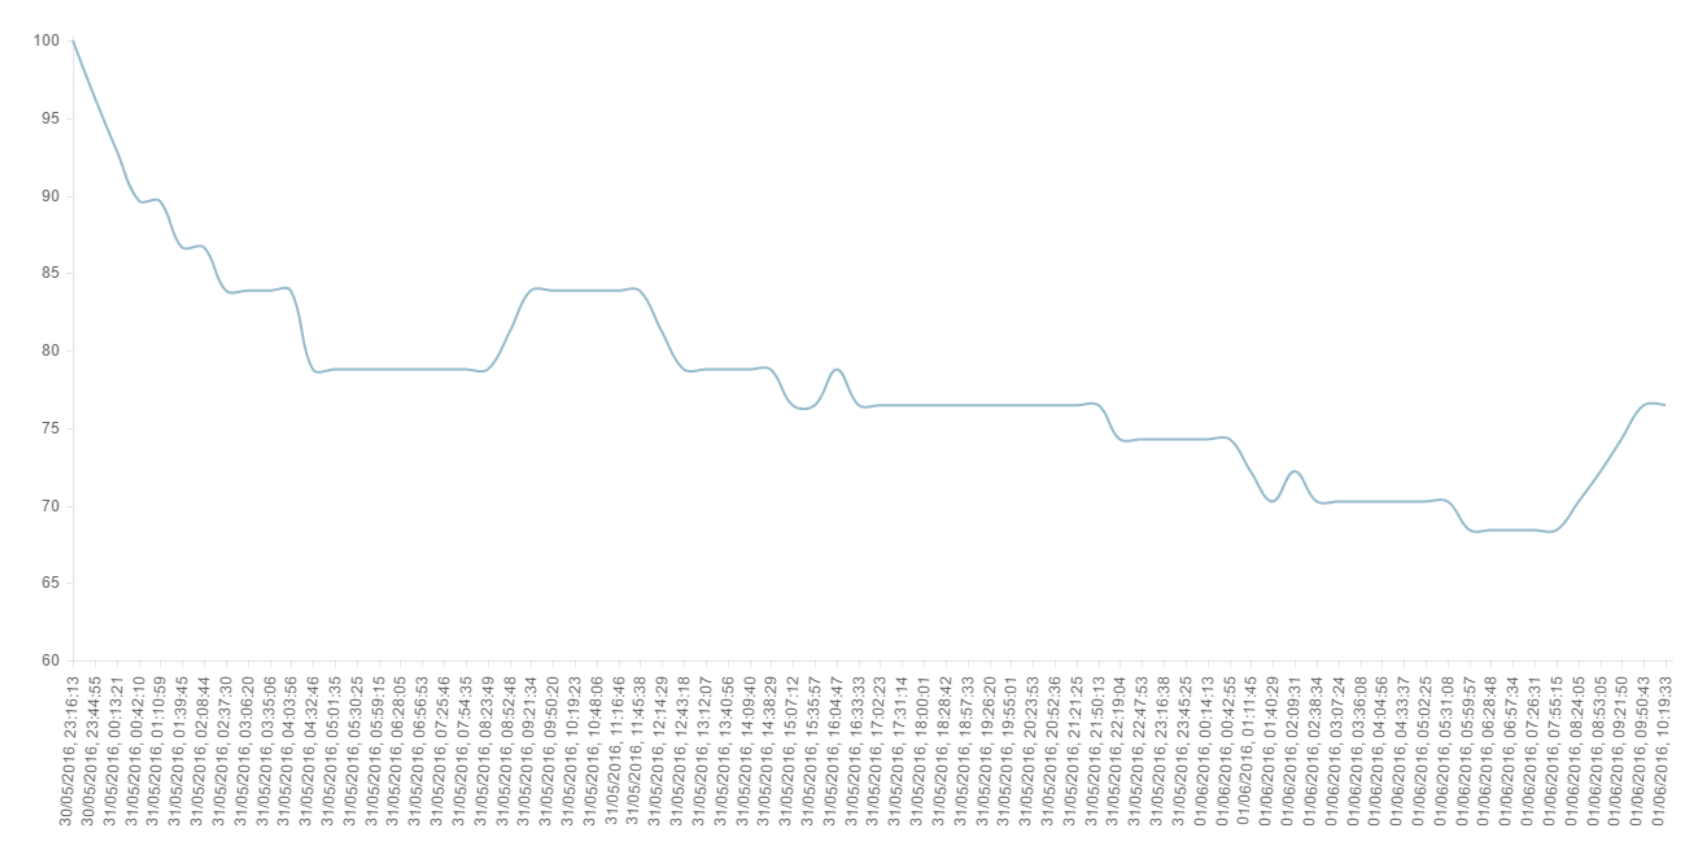
\includegraphics[width=12cm]{watergraph.png}
\end{figure}

\section{Cloud deployment}
I explored a range of options for cloud, and it is covered extensively in the cost constraint portion of the thesis. We had multiple iterations of the cloud deployment. The most like a continuous deployment/ continuous integration we came was when we implemented the front-end on azure using azure dev-ops and visual studio team services to create a hook in to our github library. However our actual long running implementation focused around much more manual processes on DigitalOcean. We had both the database, server code and front end being served from a Ubuntu server. This allowed for flexibility as well as a very low cost per month (5usd + vat). We did test hosted apps like "meteorDB" and azure web apps, but ultimately found that running our own Linux server was easier for a proof of concept project.

\section{On premise deployment}
Deployment on premise is also a good option if an area has limited coverage of internet connectivity. In fact the initial version of the proof of concept ran on an on premise deployment on my personal computer. This was also an easy and manageable way of setting up the hosting. However you are responsible for more of the deployment stack yourself. Ensuring proper networking and firewall settings is more challenging than with a cloud deployment, and normally you are not leveraging pre-built images with the necessary development tools. I also want to mention that although it is not necessarily more expensive to host this proof of concept on premise, it does have a higher up front cost as you would need to own hardware with sufficient resources to run the proof of concept.

\section{Site deployment}
 \begin{figure}[h]
\caption{Site deployment 3. iteration}
\centering
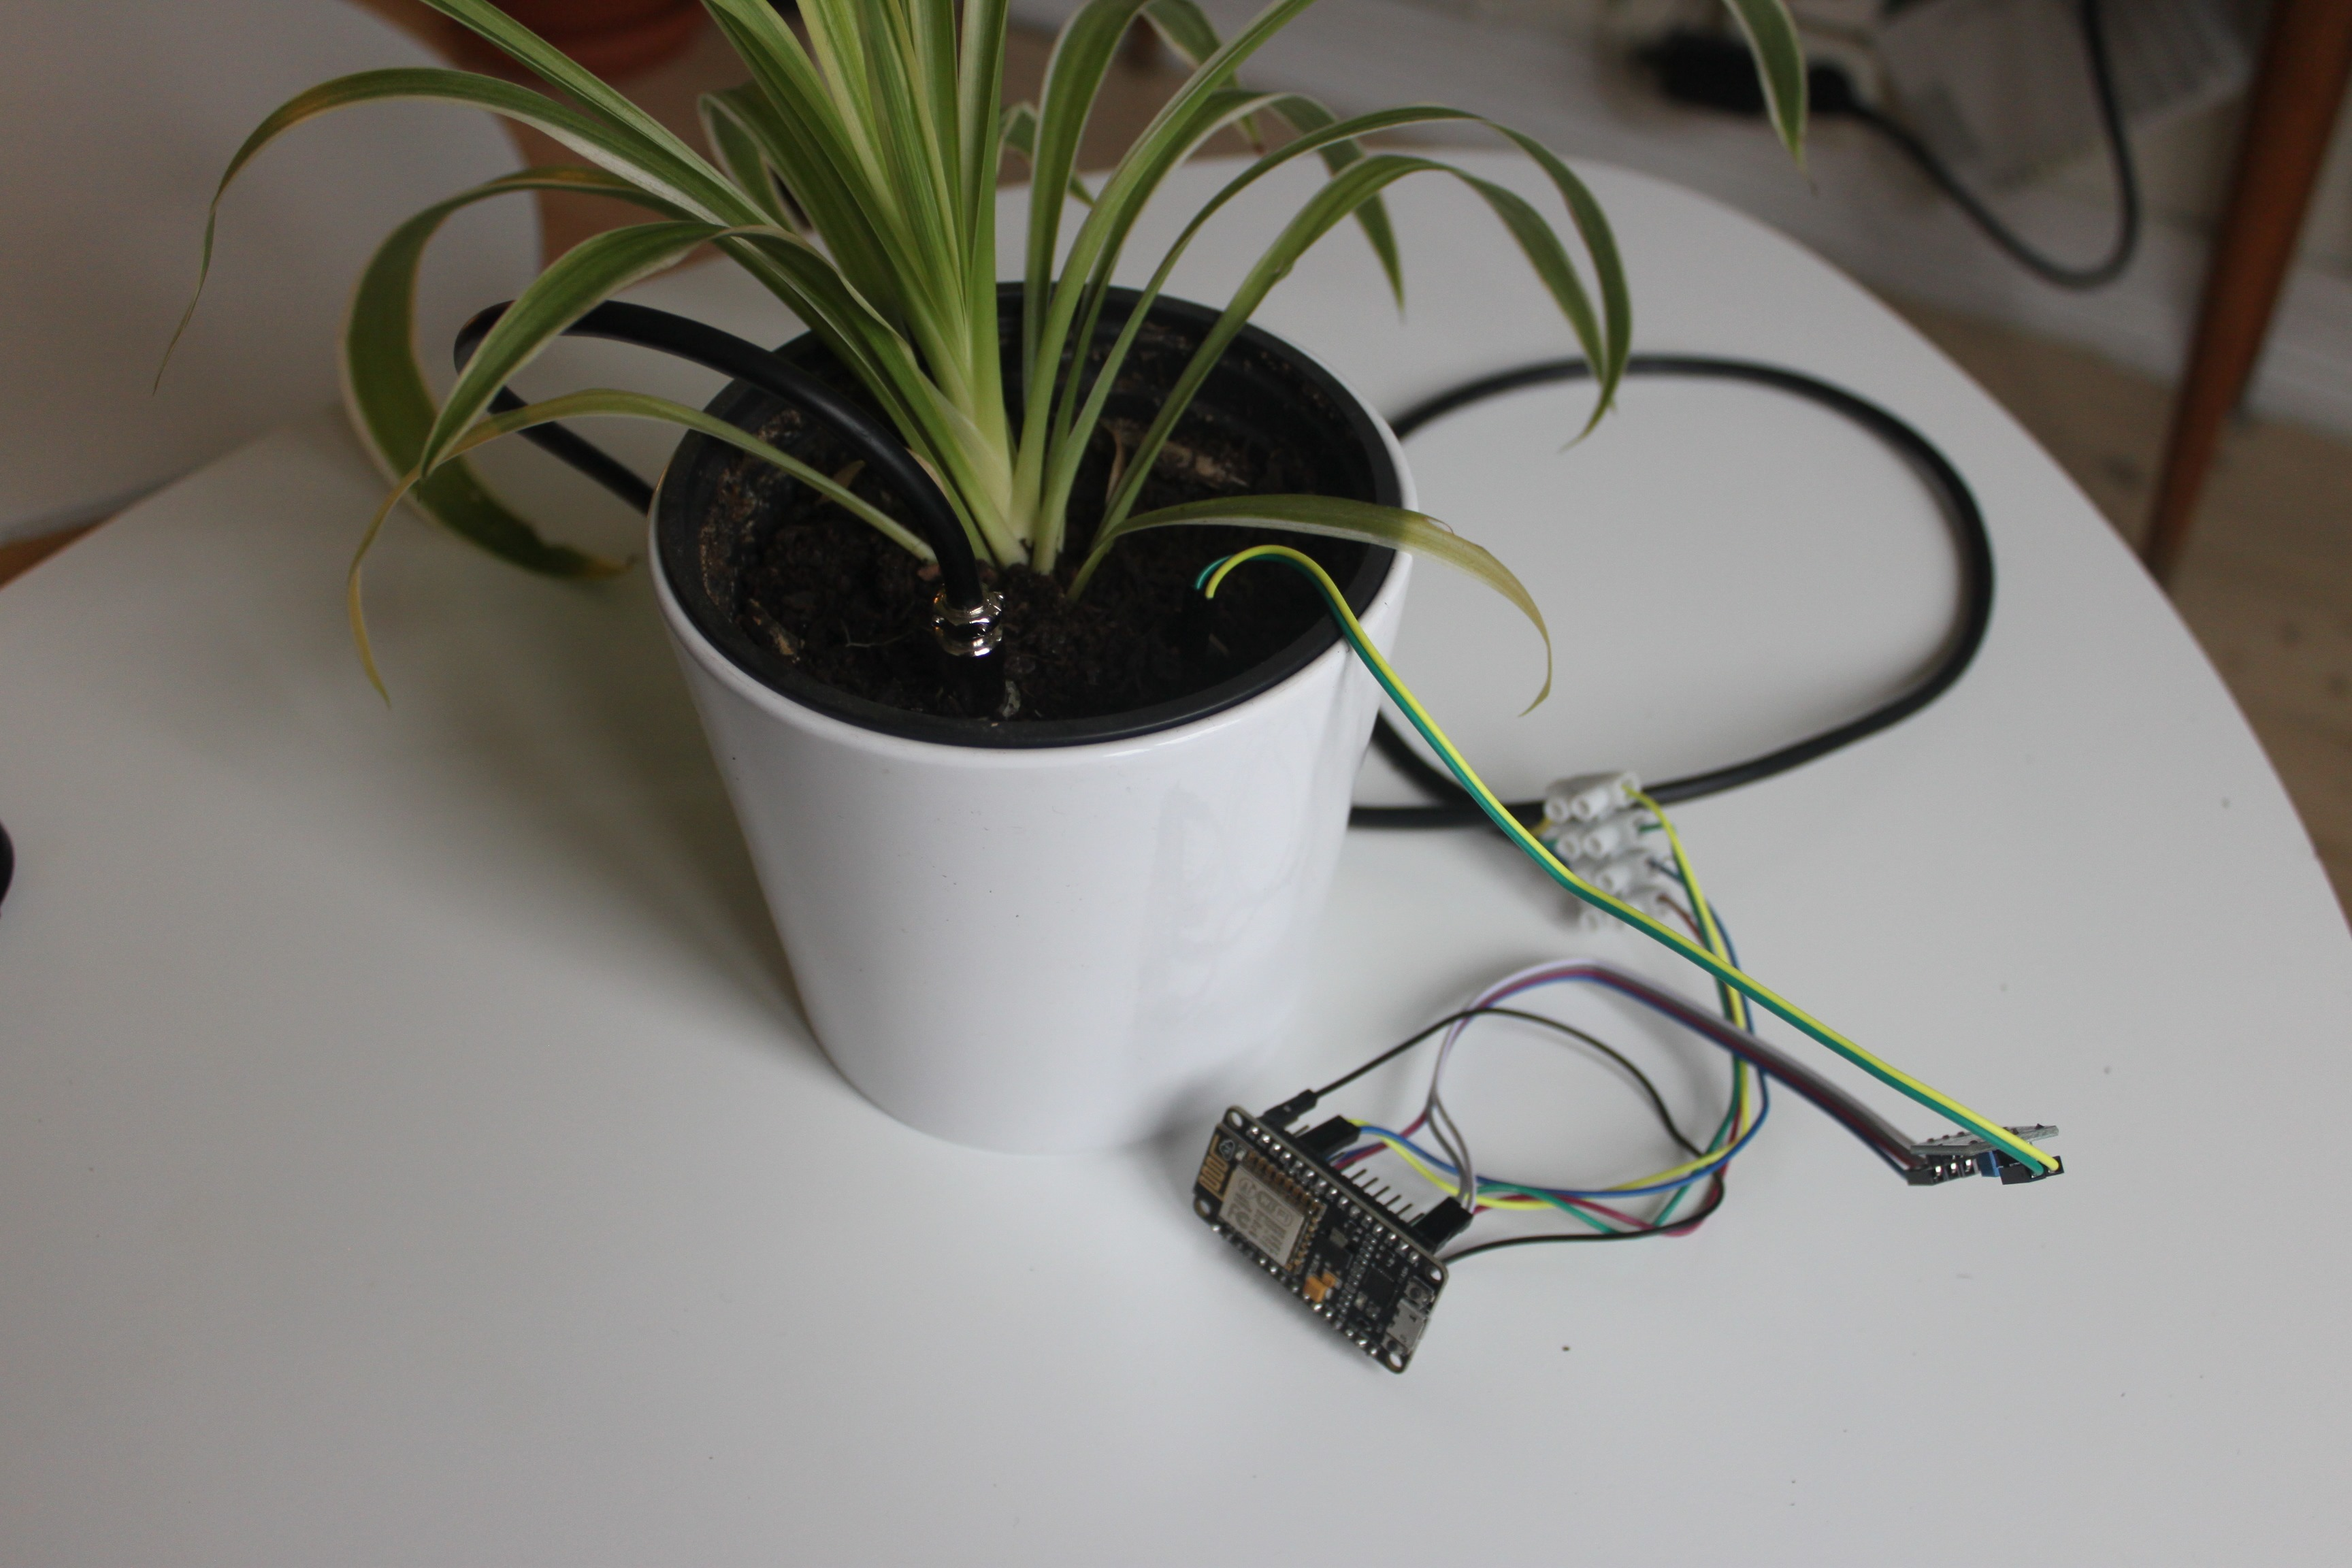
\includegraphics[width=10cm]{mcu+sensor.jpg}
\end{figure}

When we implemented the proof of concept we started off with an outdoor deployment in a greenhouse as the original idea was to also control irrigation using a threshold that would be discovered by the data. Because of this we had additional complonents in the system like a motor controller to run a pump as well as a sonic sensor to monitor the level of our tank. Although this was an interesting execise in itself we quickly relized that although fun, cortrolling the full system would give limited value to our porject. This is because through our research we started to see that the area that was lacking insight was the data on how the watering should be done. We therefore shifted focus away from the sensor housing, running pumps and building out plumbing. And instead decided to scale the project back a bit and focus on an indoor deployment. This made a few things way more simple. We no longer had to worry about water proofing the sensors. It allowed us to abandon the work on making the sensor battery powered. This allowed us to focus more on the tech platform and the architecture of the application which was more in line with the subject of research. 
\\\\
It is worth noting that we where able to run the system in the greenhouse for up to five days on battery power, and we started to see some of the challanges that would face the sensors outside in the field. One example of unexpected observation was when we noticed false readings when the sensor got heated by sunlight. This is one of the reasons we decided to purchase one of the more advanced sth11 sensors as this problem would be eliminated by the sensor reading measurements in a different way.
\\\\
In our final implementation we had the same type of sensor package deployed to five indoor plants. We collected data for 2-3 months in the fall of 2018 and this data created the grounds for the simulation program that we wrote to stress test the application.

\chapter{Conclusions and future work}

Summary of main observation, key results and conclusions, limitations of the work, suggestions for future work
\\\\
In this thesis we have explored the concepts and technologies that make up Cloud Computing and Internet of Things, we have explored in depth the configuration of Wireless Sensor Networks and we have given examples of how these technologies could be applied in agricultural scenarios to monitor soil moisture. We see from these examples that applying the knowledge of agriculturalists is crucial to the success of the efforts and that the knowledge derived from the systems help the users make the right decisions. We want to further explore how to make these technologies more efficient, how they can become more accessible to users and how they can be applied to emerging agricultural techniques like Urban Farming, Hydroponics, Aquaponics and Vertical Farming. Primarily we are interested in implementing this in a norwegian context as we have other challanges emerging with long droughts during summer in recent years and very wet periods during fall. My intuition tells us that a lot can be done to increase the yield of livestock feed crops like grass. Which has proven highly important in a Norwegian context.
\section{criteria overview}
I built a platform for gathering and visualizing data. Described as a ideal design and the implementation that followed. The initial requirements where that the platform should handle data from a large set of motes, that it should visualize the data and through the visualization provide value and insight. All this should be done at a low cost. Through the design I described how the system could scale, and by implementing the data simulation I proved that the system could handle a large amount of sensors providing data to the platform. Thus proving the solution has sufficient throughput to meet the requirement set.
\\\\
We have seen from the screenshots from the application that we are able to visualize the water consumption of a plant over time. And that the graph is easy to understand. Through this I have proved that the system is able to visualize the data, and that we can see clear trends in the data over time.
\\\\
By meeting these technical and functional requirements i believe that the system I have designed and built can aid in establishing a baseline for excess irrigation and give a clear picture of both when a farmer would need to water, but also when it is not necessary due to rainfall or other weather conditions that keep the soil at a high moisture content. However documenting this in a deployment setting would require work that is outside the scope of this thesis. It is unfortunate that I was not able to find clear numbers of a true definition of the price of gathering this data in the past, and doing a comparison of the price of each data point and the value of the information will go in to the suggested future work for this thesis Quantifying this cost reduction would have been valuable


\section{ Is sensor technology a reasonable way to address excessive irrigation}

Through this thesis this has been the central question that I set out to answer. We have looked at what excessive irrigation is, and some of the problems that can come along with excessive use of water. First we defined excessive irrigation as a management problem and not a mechanical problem with the help of the article \parencite{LILIENFELD200773}. With this knowledge we looked at the changes in ease in collecting important data that we can use in getting excessive irrigation under control. 
\\\\
My conclusion is that sensor technology undoubtedly be a good tool in the arsenal of a farmer who is concerned about water use, both from a profit and environmental perspective. I have also proved that sensor networks can be implemented and used for collecting data that used to be very hard and expensive to come by.

\section{ Can a system for monitoring water consumption be implemented with limited resource use}

In the context of this thesis we focus on resources defined as time and money. The work that was done in the proof of concept was to prove that the goal of monitoring water consumption can be done by developers with limited professional experience and knowledge about sensors and electrical engineering. Although there is a lot of trial and error involved in developing any product or software my conclusion is that this type of system can be implemented within a reasonable budget, and that building a full scale version of this system is something a small team could be able to do. Both from the ground up, like I did, or by leveraging some of the services described in this thesis.

\section{ Can such a system be implemented as a proof of concept}

Through this thesis and the wider project I have proved that a proof of concept version of the system can be implemented by one to two people using commodity hardware, open source software packages and cheap cloud solutions. I have also proved that it can be deployed, and that on can clearly see the water consumption in a plant. See fig 7.1 for hour by hour consumption example
 \begin{figure}[h]
\caption{Water consumption hour by hour}
\centering
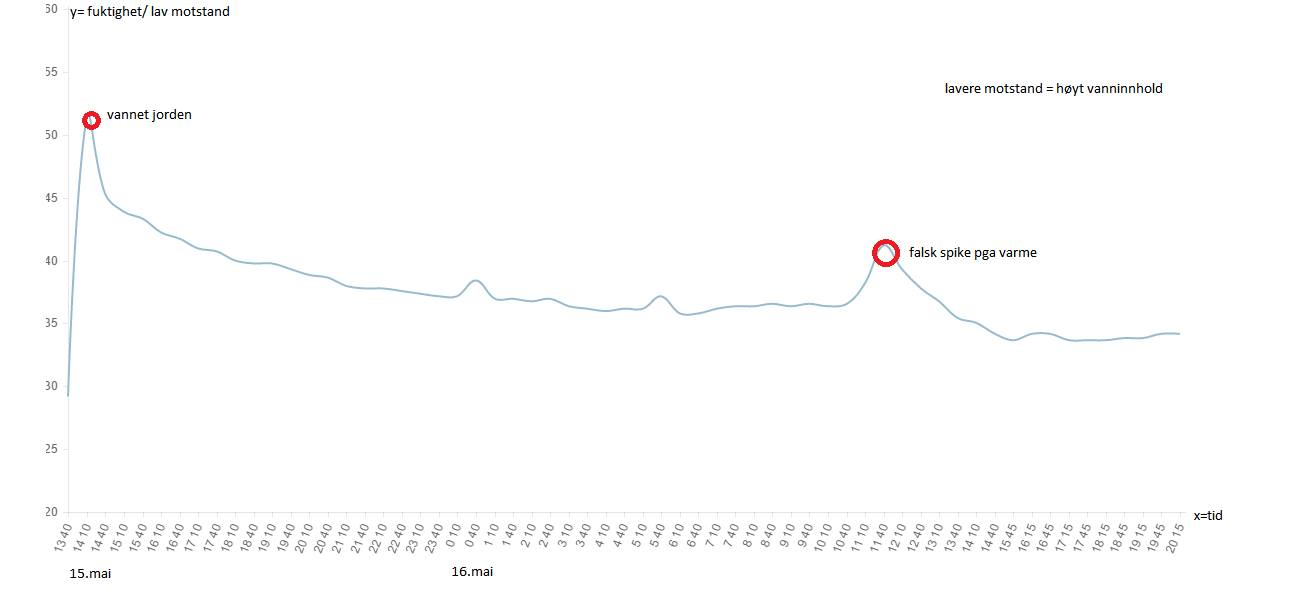
\includegraphics[width=14cm]{warter_hourbyhour.png}
\end{figure}

\section{future work}
\\\\
Something that became appareant throughout the project was that my initial assumptions regarding what factors to monitor where too limited to give  a overall picture of the health of a major farming operation. Something as basic as what depth to put the sensors at can become a  major study in itself and I would have benefitted from research and discovery around this. Although I did not go to deep in to the plant science part of the thesis we have learned that there are many factors that contribute to the state of a plant. And we have also learned that there are many factors that impact water retention in soil. Is the soil sandy, is it hard packed, what level of fertalizer is present. Learning more about the different factors, and monitoring how the different variables impact our reading would have been very interesting.
\\\\
It is also natural to think that we would want to do more with the platform I have started to develop. A few of the following items come to mind, security, automation of deployment and user and role engineering. These things where not applicable in a proof of concept scenario. But would have been a must if I ever wanted to  launch this system in a production setting.
\\\\
Mote software deployment is something I immediately saw huge problems with and the deployment model for software would have been a massive problem in a production setting. We had some ideas on how to improve this, but none that where possible to implement with the architecture that we had chosen for our project. Her I would like to invest more time in to the data transfer protocol and the network topology. I think as an example utilizing edge nodes with WIFI and running the rest of the nodes off of radio signals could reduce the points in the system where we would need to change configuration and update software. If we had problems with the http protocol implementation or needed to change or update the code, we could target the edge node as all the connectivity in one node at the edge as a gateway to our server. The goal of this suggested further work would be to achieve a greater separation of concerns, having the motes focus on data gathering and allow the edge nodes acting as gateways to deal with connectivity, data caching, uploading data. As well as limiting the number of nodes in the network that we need to change if we where to update the software or change the technology of the APIs at any point in the future.
\\\\
I have alluded to future work regarding data analysis in this thesis. I definitely believe that there is a lot of room for statistical analysis on the data sets that the sensors generate. As mentioned I have a theory that based on aggregate level data for more variables we should be able to start analyzing their relationship and see what factors have a high correlation in the model. Over time I had hoped to link this to weather data and build a model that could help in predicting and optimizing irrigation over time. This was an area where i would have liked to researched further but due to time constraints it is ending up in future work. Building a machine learning model based on the data and using factors such as sun hours and weather forecasts we should be able to say something about the rate of consumption and evaporation. Resulting in more accurate and precise irrigation use, thus contributing to reduced water usage and ensuring limitation of excessive irrigation.
\\\\
It would also be important to research the price of collecting agricultural data in the past. This would help me to quantify the cost reduction that the proof of concept gives compared to existing methods. Quantifying this reduction could have helped me underpin the conclusion of the thesis even better, and would be an important step in relating the proof of concept to the real world implementation costs of existing soulutions.

\printbibliography

\chapter{Appendix Code}
\linespread{1}

\section{init.lua}
The init .lua file is the file resposible for connecting do the wifi network and running the deep sleep function of the nodemcu.
\lstinputlisting[language=Java]{init.lua}

\section{sth11.lua}
\lstinputlisting[language=Java]{sth11.lua}

\section{main.lua}
main.lua is the file refenced in init.lua and is responsible for reading and sending the moisture data from the sensor
\lstinputlisting[language=Java]{main.lua}

\section{server.js}
Server.js is responsible for recieving and saving the data sent from the motes.
\lstinputlisting[language=Java]{server.js}

\section{index.html}
Index.html is the main file to control the front end
\lstinputlisting[language=html]{index.html}

\section{dashboard.html}
dashboard.html shows the tables and information for the water usage
\lstinputlisting[language=html]{dashboard.html}

\section{pageController.js}
pageController.js contains the controllor for managing the front end
\lstinputlisting[language=Java]{pageController.js}

\section{mote simulator.py}
Python mote simulator
\lstinputlisting[language=Python]{mote_simulator2_0.py}

\section{mote simulator.py v2}
Python mote simulator
\lstinputlisting[language=Python]{mote_simulator.py}

https://nodemcu.readthedocs.io/en/master/
\\\\
\textbf{SYN, SYN-ACK, ACK}
\\\\
Christoffer Gard Osen was my partner on this project for more than two years, but decided to leave UiO at the end of 2018. Without him i would have felt very lost through this project and would like to extend a big thanks and acknowledgment for all the good conversations, discussion and collaboration.



https://journals.plos.org/plosone/article?id=10.1371/journal.pone.0131422
\end{document}
